\documentclass{beamer}

\usepackage{beamerthemesplit}
\usetheme{Singapore} 


\input{../../include/preamble.inc} 
\input{../../include/definitions.inc} 
\input{../../include/author.inc} 

%%Copenhagen}
%%\usecolortheme{whale}
%
%\usepackage[T2A]{fontenc}
%\usepackage[utf8]{inputenc}
%\usepackage[russian]{babel}
%
%
%\usepackage{textcomp}
%\usepackage{amssymb,amsmath}
%%\usepackage{animate}
%%\usepackage{longtable}
%\usepackage{xcolor}
%
%%\usepackage{pstricks}
%
%\newcounter{N}
%
%%% Форматирование окружения itemize
%%\usepackage{ragged2e}
%%\let\olditem\item
%%\renewcommand\item{\olditem\justifying}


\title[]{Градиент и дифференциальные операторы}
%
%\author[]{ {\em Верещагин Антон Сергеевич}
%	\\
%	канд. физ.-мат. наук, доцент\\
%	\bigskip
%	Кафедра аэрогидродинамики ФЛА НГТУ
%}
%
%\newtheorem{dfn}{Определение}  
%\newtheorem{theorems}{Теорема}  
%
%\newcommand{\Rn}{\mathrm{R}^n}
%\newcommand{\Sm}{\mathrm{S}^m}
%\newcommand{\Ql}{\mathrm{Q}^l}
%
%\newcommand{\Rd}[1]{\mathbb{R}^{#1}}
%\newcommand{\Vn}{\mathrm{V}^n}
%
%\newcommand{\oper}[1]{{\bf #1}}
%\newcommand{\basis}[1]{\vec{\bf #1}}
%\newcommand{\dt}[1]{\frac{d #1}{dt}}
%\newcommand{\dtds}[1]{\displaystyle\frac{d #1}{dt}}
%\newcommand{\ds}[1]{\frac{d #1}{ds}}
%\newcommand{\dsds}[1]{\displaystyle\frac{d #1}{ds}}
%\newcommand{\dsd}[1]{\frac{d^2 #1}{ds^2}}
%\newcommand{\pdt}[1]{\frac{\partial #1}{\partial t}}
%\newcommand{\pds}[1]{\frac{\partial #1}{\partial s}}
%\newcommand{\pdx}[1]{\frac{\partial #1}{\partial x}}
%\newcommand{\pdy}[1]{\frac{\partial #1}{\partial y}}
%\newcommand{\pdz}[1]{\frac{\partial #1}{\partial z}}
%\newcommand{\pdxds}[1]{\displaystyle\frac{\partial #1}{\partial x}}
%\newcommand{\pdyds}[1]{\displaystyle\frac{\partial #1}{\partial y}}
%\newcommand{\pdzds}[1]{\displaystyle\frac{\partial #1}{\partial z}}
%\newcommand{\pdn}[1]{\frac{\partial #1}{\partial n}}
%\newcommand{\grad}[1]{{\rm grad}\, #1}


\begin{document}

\frame[plain]{\titlepage}


\frame[plain]{
\frametitle{Аннотация}
\parbox{\textwidth}{Градиент и его свойства. Потенциальный вектор и его свойства. Градиент вектора по вектору. Субстанциональная производная.
}
}

\frame{
\frametitle{Производная вдоль кривой}

\parbox{\textwidth}{
\scriptsize
Рассмотрим скалярное поле функции $\varphi(\vec{r})=\varphi(x,y,z)$. \pause  Проведём некоторую кривую $L$, параметризованную с помощью параметра $s$ -- расстояния до некоторой точки $M$:
\[ 
x=x(s),\quad y=y(s),\quad z=z(s). 
\] \pause 
Тогда производная вдоль кривой имеет вид:
\[ 
\ds{}\varphi(x(s),y(s),z(s))=\pdx{\varphi}\ds{x}+\pdy{\varphi}\ds{y}+\pdz{\varphi}\ds{z}.
\] \pause 
Обыкновенные производные в равенстве -- направляющие косинусы ($\vec{s}$ -- единичный вектор касательных)
\[ 
\ds{x}=\cos(\vec{s},x),\quad \ds{y}=\cos(\vec{s},y),\quad \ds{z}=\cos(\vec{s},z), 
\]  \pause 
то
\[ 
\ds{\varphi}=\pdx{\varphi}\cos(\vec{s},x)+\pdy{\varphi}\cos(\vec{s},y)+\pdz{\varphi}\cos(\vec{s},z).
\] \pause 
Таким образом, $ \dsds{\varphi} $ -- проекция вектора $(\pdx{\varphi},\pdy{\varphi},\pdz{\varphi})$ на вектор $\vec{s}$.
}
}

\frame{
\frametitle{Определение градиента}

\begin{dfn}
\parbox{\textwidth}{
Вектор с компонентами $(\pdx{\varphi},\pdy{\varphi},\pdz{\varphi})$ называется \alert{градиентом функции} $ \varphi $ в точке $M$ и обозначается $ \grad{\varphi} $.
}
\end{dfn} \pause 

\bigskip
\parbox{\textwidth}{
Отсюда
\[ 
\grad{\varphi}=\basis{i}\pdx{\varphi}+\basis{j}\pdy{\varphi}+\basis{k}\pdz{\varphi}.
\] \pause 
Длина вектора
\[ 
|\grad{\varphi}|=\sqrt{\left(\pdx{\varphi}\right)^2+\left(\pdy{\varphi}\right)^2+\left(\pdz{\varphi}\right)^2}.
\]
}
}

\frame{
\frametitle{Альтернативное определение градиента}
\parbox{\textwidth}{
Еще одно выражение для производной вдоль направления $ \vec{s} $: 
\[ 
\ds{\varphi}= \pause \vec{s}\cdot\grad{\varphi}= \pause |\grad{\varphi}|\, \cos(\grad{\varphi},\vec{s}),
\]
из которого вытекает следующее определение:
} \pause 

\begin{dfn}
\parbox{\textwidth}{
\alert{Градиентом функции} $\varphi$ называется вектор, имеющий направление быстрейшего роста функции $ \varphi $ и по величине равный производной в этом направлении.
}
\end{dfn}

}


\frame{
\frametitle{Оператор набла или оператор Гамильтона}
\begin{dfn}
\parbox{\textwidth}{

Дифференциальный оператор 
\[ 
\nabla=\basis{i}\pdx{}+\basis{j}\pdy{}+\basis{k}\pdz{}
\]
называется \alert{наблой} или \alert{оператором Гамильтона}.
}
\end{dfn} \pause 

\medskip
\parbox{\textwidth}{
В терминах оператора набла градиент функции можно записать в виде:
\[ 
\nabla\varphi=\basis{i}\pdx{\varphi}+\basis{j}\pdy{\varphi}+\basis{k}\pdz{\varphi}.
\]
}
}

\frame{
\frametitle{Поверхность уровня}

\begin{columns}
\begin{column}{0.3\textwidth}
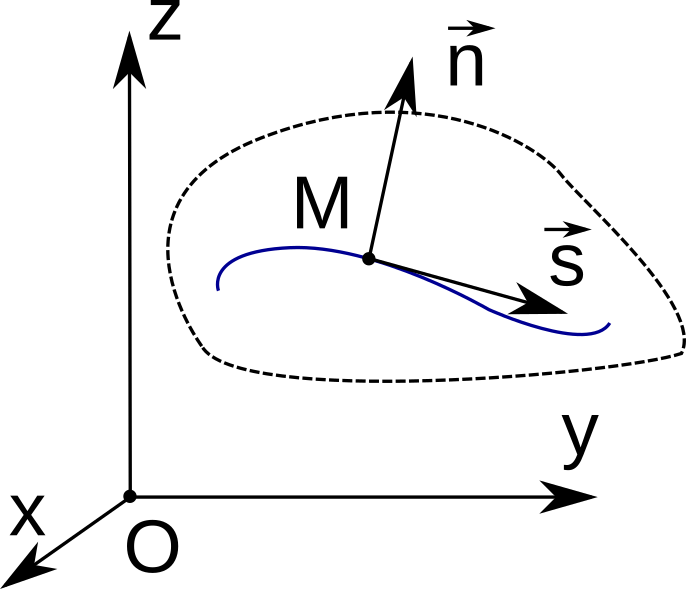
\includegraphics[width=\textwidth]{../img/level_surface.png}
\end{column} \pause 
\begin{column}{0.7\textwidth}
\parbox{\textwidth}{
Через произвольную точку $M$ проведем поверхность уровня 
\[
\varphi(x,y,z)={\rm const}.
\] \pause 
Т.к. производная вдоль любой кривой, лежащей на поверхности уровня, от $\varphi(x,y,z)$  равна
}
\end{column}
\end{columns}
\parbox{\textwidth}{
{\scriptsize
\[
\begin{array}{c}
\dsds{}\varphi(x(s),y(s),z(s)) =  \pause \lim_{\Delta s \to 0}
\displaystyle\frac{\varphi(x(s+\Delta s),y(s+\Delta s),z(s+\Delta s))-\varphi(x(s),y(s),z(s))}{\Delta s}=  \pause \\
= \grad{\varphi} \cdot \vec{s} =  \pause 0.
\end{array}
\]}
Следовательно градиент ортогонален касательной плоскости в т. $M$,  \pause и
\alert{
\[ 
\grad{\varphi}=\pdn{\varphi}\vec{n},
\]}
где $\vec{n}$ -- вектор единичной нормали к поверхности уровня.
}

}

\frame{
\frametitle{Поверхность и трубка тока}
\small

\begin{dfn}
\parbox{\textwidth}{
\alert{Поверхностью тока} вектора $\vec{v}$ называется  поверхность, образованная линиями тока, проходящими через некоторую наперед заданную кривую.
}
\end{dfn} \pause 

\begin{dfn}
\parbox{\textwidth}{
\alert{Трубкой тока} вектора $\vec{v}$ называется  часть пространства, заключенная внутри поверхности тока, образованной замкнутой кривой.
}
\end{dfn} \pause 

\bigskip
\parbox{\textwidth}{
Пусть векторные линии для поля скоростей $ \vec{v}(x,y,z) $ определяются соотношением 
\[
\Phi(x,y,z)=0.
\] \pause 
По определению поверхности тока $\vec{v}$ является касательным в любой точке этой поверхности и следовательно
\[ 
\vec{v}\cdot\grad{\Phi}=0,
\]
что является уравнением поверхности тока.
}
}

\frame{
\frametitle{Представление дифференциала функции через градиент}
\parbox{\textwidth}{
Пусть 
\[ 
d\vec{r}=\basis{i}dx+\basis{j}dy+\basis{k}dz,
\] \pause 
тогда 
\[
\begin{array}{c}
d\vec{r}\cdot\grad{\varphi}= \pause 
\left(\basis{i}dx+\basis{j}dy+\basis{k}dz\right)\cdot
\left(\basis{i}\pdxds{\varphi}+\basis{j}\pdyds{\varphi}+\basis{k}\pdzds{\varphi}\right)=\\ \pause 
=\pdxds{\varphi}dx+\pdyds{\varphi}dy+\pdzds{\varphi}dz= \pause d\varphi
\end{array} 
\] \pause 

Таким образом для произвольного вектора $d\vec{r}$
\alert{\[ d\varphi=d\vec{r}\cdot\grad{\varphi}. \]}
}
}

\frame{
\frametitle{Теорема о градиенте}
\begin{theorems}[о градиенте функции]\normalfont
\parbox{\textwidth}{
Если для некоторой скалярной функции $ \varphi(\vec{r}) $ найдется такой вектор $ \vec{a} $, \pause  что для произвольных векторов $ d\vec{r} $ справедливо равенство
\[
d\varphi=d\vec{r}\cdot\vec{a},
\] \pause 
то вектор $ \vec{a} $ есть градиент функции $ \varphi(\vec{r}): \vec{a}=\grad{\varphi} $.
}
\end{theorems} \pause 

\begin{proof}
\parbox{\textwidth}{
Из равенства для полного дифференциала $d\varphi$ вычтем равенство из условия теоремы, тогда
\[ 0=d\vec{r}\cdot(\vec{a}-\grad{\varphi}). \] \pause 
В силу произвольности $ d\vec{r} $ $ \vec{a}=\grad{\varphi} $.


}
\end{proof}
}


\frame{
\frametitle{Пример}
\begin{exampleblock}{\parbox{\textwidth}{Градиент функции, зависящий только от расстояния до начала координат}}
\parbox{\textwidth}{
Пусть $ \varphi=\varphi(r) $, где $r = \sqrt{x^2+y^2+z^2}$. \pause 

Рассмотрим выражение
\[
%\begin{array}{c}
2\vec{r}\cdot d\vec{r}= \pause 
d(\vec{r}\cdot\vec{r})=  \pause 
dr^2= \pause 2rdr
\quad \Rightarrow \quad  \pause 
dr=d\vec{r}\cdot\frac{\vec{r}}{r}.
%\end{array}
\]
Тогда
\[
d\varphi= \pause 
\varphi'(r) dr=  \pause 
d\vec{r}\cdot\frac{\varphi'(r)}{r}\vec{r}.
\] \pause 

\medskip
По теореме о градиенте 
\alert{
\[
\grad{r} = \frac{\vec{r}}{r},\quad \pause 
\grad{\varphi} = \frac{\varphi'(r)}{r}\vec{r}.
\]
}

}
\end{exampleblock}


}

\frame{
\frametitle{Потенциальный вектор}
\begin{dfn}
\parbox{\textwidth}{
Вектор, являющийся градиентом некоторой скалярной функции, называется \alert{потенциальным вектором},  \pause а поле такого вектора -- \alert{потенциальным} и сама скалярная функция \alert{потенциалом}.
}
\end{dfn} \pause 

\medskip
\begin{exampleblock}{Пример потенциального поля $\vec{a}(\vec{r})$}
Для следующих функций $\vec{a}=\grad{\varphi}$: \pause 
\begin{itemize}
\item $\vec{a}(\vec{r})=x\basis{i}+y\basis{j}+z\basis{k}=\vec{r}$,  \pause $\varphi(\vec{r})=1/2(x^2+y^2+z^2)=r^2/2$; \pause 
\item $\vec{a}(\vec{r})= \vec{r}/r$,  \pause $\varphi(\vec{r})=r$.
\end{itemize}
\end{exampleblock}
}


\frame{
\frametitle{Линейный интеграл от векторной функции вдоль кривой}
\begin{columns}
\begin{column}{0.4\textwidth}
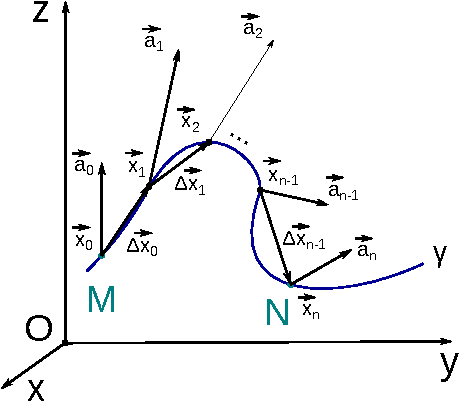
\includegraphics[width=\textwidth]{../img/pdf/integral.pdf}
%%LaTeX with PSTricks extensions
%%Creator: inkscape 0.91
%%Please note this file requires PSTricks extensions
\psset{xunit=.5pt,yunit=.5pt,runit=.5pt}
\begin{pspicture}(275.47444621,240.89019355)
{
\newrgbcolor{curcolor}{0 0 0}
\pscustom[linewidth=1,linecolor=curcolor]
{
\newpath
\moveto(39.16221,34.17174592)
\lineto(39.41475,238.98017592)
}
}
{
\newrgbcolor{curcolor}{0 0 0}
\pscustom[linestyle=none,fillstyle=solid,fillcolor=curcolor]
{
\newpath
\moveto(39.40981778,234.98017896)
\lineto(41.40735016,232.97771437)
\lineto(39.41598305,239.98017516)
\lineto(37.4073532,232.98264659)
\lineto(39.40981778,234.98017896)
\closepath
}
}
{
\newrgbcolor{curcolor}{0 0 0}
\pscustom[linewidth=0.5,linecolor=curcolor]
{
\newpath
\moveto(39.40981778,234.98017896)
\lineto(41.40735016,232.97771437)
\lineto(39.41598305,239.98017516)
\lineto(37.4073532,232.98264659)
\lineto(39.40981778,234.98017896)
\closepath
}
}
{
\newrgbcolor{curcolor}{0 0 0}
\pscustom[linewidth=1,linecolor=curcolor]
{
\newpath
\moveto(39.09908,34.67682592)
\lineto(270.12379,35.74825592)
}
}
{
\newrgbcolor{curcolor}{0 0 0}
\pscustom[linestyle=none,fillstyle=solid,fillcolor=curcolor]
{
\newpath
\moveto(266.12383302,35.7297052)
\lineto(264.13312988,33.72045135)
\lineto(271.12377925,35.7528936)
\lineto(264.11457917,37.72040834)
\lineto(266.12383302,35.7297052)
\closepath
}
}
{
\newrgbcolor{curcolor}{0 0 0}
\pscustom[linewidth=0.5,linecolor=curcolor]
{
\newpath
\moveto(266.12383302,35.7297052)
\lineto(264.13312988,33.72045135)
\lineto(271.12377925,35.7528936)
\lineto(264.11457917,37.72040834)
\lineto(266.12383302,35.7297052)
\closepath
}
}
{
\newrgbcolor{curcolor}{0 0 0}
\pscustom[linewidth=1,linecolor=curcolor]
{
\newpath
\moveto(38.94983,34.75845592)
\lineto(1.55612,8.14398592)
}
}
{
\newrgbcolor{curcolor}{0 0 0}
\pscustom[linestyle=none,fillstyle=solid,fillcolor=curcolor]
{
\newpath
\moveto(4.8149784,10.46343454)
\lineto(5.28468329,13.25258806)
\lineto(0.7414054,7.56412376)
\lineto(7.60413191,9.99372965)
\lineto(4.8149784,10.46343454)
\closepath
}
}
{
\newrgbcolor{curcolor}{0 0 0}
\pscustom[linewidth=0.5,linecolor=curcolor]
{
\newpath
\moveto(4.8149784,10.46343454)
\lineto(5.28468329,13.25258806)
\lineto(0.7414054,7.56412376)
\lineto(7.60413191,9.99372965)
\lineto(4.8149784,10.46343454)
\closepath
}
}
{
\newrgbcolor{curcolor}{0 0 0}
\pscustom[linestyle=none,fillstyle=solid,fillcolor=curcolor]
{
\newpath
\moveto(30.68822028,43.51313041)
\curveto(30.68822028,41.89447807)(30.37694099,40.47724174)(29.75438239,39.26142143)
\curveto(29.13914802,38.04560111)(28.25291755,37.11176322)(27.09569099,36.45990776)
\curveto(25.93846442,35.80805229)(24.57249763,35.48212455)(22.9977906,35.48212455)
\curveto(21.40843513,35.48212455)(20.03514411,35.80439018)(18.87791755,36.44892143)
\curveto(17.72801521,37.09345268)(16.84910896,38.02362846)(16.2411988,39.23944877)
\curveto(15.63328864,40.4625933)(15.32933356,41.88715385)(15.32933356,43.51313041)
\curveto(15.32933356,45.98871635)(16.0068238,47.9223101)(17.36180427,49.31391166)
\curveto(18.71678474,50.71283744)(20.60277106,51.41230033)(23.01976325,51.41230033)
\curveto(24.59447028,51.41230033)(25.96043708,51.09735893)(27.11766364,50.46747611)
\curveto(28.27489021,49.84491752)(29.15745856,48.9367144)(29.76536872,47.74286674)
\curveto(30.3806031,46.54901908)(30.68822028,45.13910697)(30.68822028,43.51313041)
\closepath
\moveto(28.5458863,43.51313041)
\curveto(28.5458863,45.43939994)(28.06248786,46.95185111)(27.09569099,48.05048393)
\curveto(26.13621833,49.14911674)(24.77757575,49.69843315)(23.01976325,49.69843315)
\curveto(21.24730231,49.69843315)(19.87767341,49.15644096)(18.91087653,48.07245658)
\curveto(17.94407966,46.98847221)(17.46068122,45.46869682)(17.46068122,43.51313041)
\curveto(17.46068122,41.57221244)(17.94774177,40.0304644)(18.92186286,38.88788627)
\curveto(19.90330817,37.75263236)(21.26195075,37.18500541)(22.9977906,37.18500541)
\curveto(24.78489997,37.18500541)(26.15452888,37.73432182)(27.10667731,38.83295463)
\curveto(28.06614997,39.93891166)(28.5458863,41.49897026)(28.5458863,43.51313041)
\closepath
}
}
{
\newrgbcolor{curcolor}{0 0 0}
\pscustom[linestyle=none,fillstyle=solid,fillcolor=curcolor]
{
\newpath
\moveto(24.71327521,0.00000785)
\lineto(21.51625373,4.87793754)
\lineto(18.29725959,0.00000785)
\lineto(16.16591193,0.00000785)
\lineto(20.39564826,6.10840629)
\lineto(16.36366584,11.88721488)
\lineto(18.54994514,11.88721488)
\lineto(21.51625373,7.26197074)
\lineto(24.46058967,11.88721488)
\lineto(26.66884162,11.88721488)
\lineto(22.6368592,6.13037895)
\lineto(26.92152717,0.00000785)
\lineto(24.71327521,0.00000785)
\closepath
}
}
{
\newrgbcolor{curcolor}{0 0 0}
\pscustom[linestyle=none,fillstyle=solid,fillcolor=curcolor]
{
\newpath
\moveto(266.36677863,11.50666068)
\curveto(265.82478645,11.50666068)(265.37068488,11.54694389)(265.00447395,11.62751029)
\lineto(265.00447395,13.11066459)
\curveto(265.28279426,13.06671928)(265.59041145,13.04474662)(265.92732551,13.04474662)
\curveto(267.15779426,13.04474662)(268.13191535,13.94928764)(268.84968879,15.75836967)
\lineto(269.03645637,16.23078178)
\lineto(264.3233216,28.06305717)
\lineto(266.4326966,28.06305717)
\lineto(268.93757941,21.49323295)
\curveto(268.97420051,21.39069389)(269.01814582,21.26618217)(269.06941535,21.11969779)
\curveto(269.12068488,20.98053764)(269.2854798,20.50446342)(269.56380012,19.69147514)
\curveto(269.84212043,18.87848686)(269.99226691,18.42438529)(270.01423957,18.32917045)
\lineto(270.78328254,20.49347709)
\lineto(273.3870423,28.06305717)
\lineto(275.47444465,28.06305717)
\lineto(270.90413215,16.17585014)
\curveto(270.41340949,14.90876029)(269.95564582,13.96759818)(269.53084113,13.35236381)
\curveto(269.10603645,12.72980522)(268.63362434,12.26837943)(268.1136048,11.96808647)
\curveto(267.60090949,11.66046928)(267.0186341,11.50666068)(266.36677863,11.50666068)
\closepath
}
}
{
\newrgbcolor{curcolor}{0 0 0}
\pscustom[linestyle=none,fillstyle=solid,fillcolor=curcolor]
{
\newpath
\moveto(20.30351569,227.65967582)
\lineto(20.30351569,229.16480277)
\lineto(26.95024421,238.01978324)
\lineto(20.67705085,238.01978324)
\lineto(20.67705085,239.54688285)
\lineto(29.2903321,239.54688285)
\lineto(29.2903321,238.0417559)
\lineto(22.63261726,229.18677543)
\lineto(29.52104499,229.18677543)
\lineto(29.52104499,227.65967582)
\lineto(20.30351569,227.65967582)
\closepath
}
}
{
\newrgbcolor{curcolor}{0 0 0}
\pscustom[linestyle=none,fillstyle=solid,fillcolor=curcolor]
{
\newpath
\moveto(40.82871439,34.90467094)
\curveto(40.82871439,33.93393019)(40.04177353,33.14698933)(39.07103278,33.14698933)
\curveto(38.10029204,33.14698933)(37.31335118,33.93393019)(37.31335118,34.90467094)
\curveto(37.31335118,35.87541169)(38.10029204,36.66235255)(39.07103278,36.66235255)
\curveto(40.04177353,36.66235255)(40.82871439,35.87541169)(40.82871439,34.90467094)
\closepath
}
}
{
\newrgbcolor{curcolor}{0 0 0}
\pscustom[linewidth=0.48463672,linecolor=curcolor]
{
\newpath
\moveto(40.82871439,34.90467094)
\curveto(40.82871439,33.93393019)(40.04177353,33.14698933)(39.07103278,33.14698933)
\curveto(38.10029204,33.14698933)(37.31335118,33.93393019)(37.31335118,34.90467094)
\curveto(37.31335118,35.87541169)(38.10029204,36.66235255)(39.07103278,36.66235255)
\curveto(40.04177353,36.66235255)(40.82871439,35.87541169)(40.82871439,34.90467094)
\closepath
}
}
{
\newrgbcolor{curcolor}{0 0 0.57254905}
\pscustom[linewidth=1,linecolor=curcolor]
{
\newpath
\moveto(52.17372,77.92685592)
\curveto(52.17372,77.92685592)(74.48174,99.55314592)(86.45943,122.92685592)
\curveto(118.45287,185.36006592)(162.02507,141.55808592)(155.53222,124.01995592)
\curveto(132.306,57.06664592)(203.03242,58.44487592)(253.95943,82.39114592)
}
}
{
\newrgbcolor{curcolor}{0 0 0}
\pscustom[linestyle=none,fillstyle=solid,fillcolor=curcolor]
{
\newpath
\moveto(91.16614725,128.74048637)
\curveto(91.16614725,127.76974562)(90.37920639,126.98280476)(89.40846564,126.98280476)
\curveto(88.4377249,126.98280476)(87.65078404,127.76974562)(87.65078404,128.74048637)
\curveto(87.65078404,129.71122712)(88.4377249,130.49816798)(89.40846564,130.49816798)
\curveto(90.37920639,130.49816798)(91.16614725,129.71122712)(91.16614725,128.74048637)
\closepath
}
}
{
\newrgbcolor{curcolor}{0 0 0}
\pscustom[linewidth=0.48463672,linecolor=curcolor]
{
\newpath
\moveto(91.16614725,128.74048637)
\curveto(91.16614725,127.76974562)(90.37920639,126.98280476)(89.40846564,126.98280476)
\curveto(88.4377249,126.98280476)(87.65078404,127.76974562)(87.65078404,128.74048637)
\curveto(87.65078404,129.71122712)(88.4377249,130.49816798)(89.40846564,130.49816798)
\curveto(90.37920639,130.49816798)(91.16614725,129.71122712)(91.16614725,128.74048637)
\closepath
}
}
{
\newrgbcolor{curcolor}{0 0 0}
\pscustom[linestyle=none,fillstyle=solid,fillcolor=curcolor]
{
\newpath
\moveto(157.88285257,126.5674517)
\curveto(157.88285257,125.59671095)(157.09591171,124.80977009)(156.12517097,124.80977009)
\curveto(155.15443022,124.80977009)(154.36748936,125.59671095)(154.36748936,126.5674517)
\curveto(154.36748936,127.53819245)(155.15443022,128.32513331)(156.12517097,128.32513331)
\curveto(157.09591171,128.32513331)(157.88285257,127.53819245)(157.88285257,126.5674517)
\closepath
}
}
{
\newrgbcolor{curcolor}{0 0 0}
\pscustom[linewidth=0.48463672,linecolor=curcolor]
{
\newpath
\moveto(157.88285257,126.5674517)
\curveto(157.88285257,125.59671095)(157.09591171,124.80977009)(156.12517097,124.80977009)
\curveto(155.15443022,124.80977009)(154.36748936,125.59671095)(154.36748936,126.5674517)
\curveto(154.36748936,127.53819245)(155.15443022,128.32513331)(156.12517097,128.32513331)
\curveto(157.09591171,128.32513331)(157.88285257,127.53819245)(157.88285257,126.5674517)
\closepath
}
}
{
\newrgbcolor{curcolor}{0 0.50196081 0.50196081}
\pscustom[linestyle=none,fillstyle=solid,fillcolor=curcolor]
{
\newpath
\moveto(66.55870368,53.25861381)
\lineto(66.55870368,63.58576225)
\curveto(66.55870368,64.72834037)(66.59166267,65.82697318)(66.65758063,66.88166068)
\curveto(66.29869392,65.57062553)(65.97642829,64.5452349)(65.69078376,63.80548881)
\lineto(61.69176032,53.25861381)
\lineto(60.21959235,53.25861381)
\lineto(56.16563728,63.80548881)
\lineto(55.5504029,65.67316459)
\lineto(55.18785407,66.88166068)
\lineto(55.22081306,65.66217826)
\lineto(55.26475837,63.58576225)
\lineto(55.26475837,53.25861381)
\lineto(53.39708259,53.25861381)
\lineto(53.39708259,68.73835014)
\lineto(56.15465095,68.73835014)
\lineto(60.27452399,58.00470756)
\curveto(60.42100837,57.57257865)(60.56016853,57.10749076)(60.69200446,56.60944389)
\curveto(60.83116462,56.11872123)(60.92271735,55.76349662)(60.96666267,55.54377006)
\curveto(61.02525642,55.83673881)(61.14610603,56.27985404)(61.32921149,56.87311576)
\curveto(61.51964118,57.4737017)(61.64781501,57.85089897)(61.71373298,58.00470756)
\lineto(65.75670173,68.73835014)
\lineto(68.44835212,68.73835014)
\lineto(68.44835212,53.25861381)
\lineto(66.55870368,53.25861381)
\closepath
}
}
{
\newrgbcolor{curcolor}{0 0.50196081 0.50196081}
\pscustom[linestyle=none,fillstyle=solid,fillcolor=curcolor]
{
\newpath
\moveto(170.1481507,45.57227348)
\lineto(161.8644593,58.75586723)
\lineto(161.91939094,57.6901934)
\lineto(161.97432258,55.8554766)
\lineto(161.97432258,45.57227348)
\lineto(160.1066468,45.57227348)
\lineto(160.1066468,61.05200981)
\lineto(162.54561164,61.05200981)
\lineto(170.91719367,47.78052543)
\curveto(170.82930305,49.21607231)(170.78535773,50.25611137)(170.78535773,50.90064262)
\lineto(170.78535773,61.05200981)
\lineto(172.67500617,61.05200981)
\lineto(172.67500617,45.57227348)
\lineto(170.1481507,45.57227348)
\closepath
}
}
{
\newrgbcolor{curcolor}{0 0 0}
\pscustom[linestyle=none,fillstyle=solid,fillcolor=curcolor]
{
\newpath
\moveto(49.68516853,93.12928031)
\lineto(47.90904548,95.83924125)
\lineto(46.1207154,93.12928031)
\lineto(44.93663337,93.12928031)
\lineto(47.28648688,96.522835)
\lineto(45.04649665,99.73328422)
\lineto(46.26109626,99.73328422)
\lineto(47.90904548,97.16370414)
\lineto(49.54478767,99.73328422)
\lineto(50.77159431,99.73328422)
\lineto(48.53160407,96.53504203)
\lineto(50.91197517,93.12928031)
\lineto(49.68516853,93.12928031)
\closepath
}
}
{
\newrgbcolor{curcolor}{0 0 0}
\pscustom[linestyle=none,fillstyle=solid,fillcolor=curcolor]
{
\newpath
\moveto(55.24760749,93.42621635)
\curveto(55.24760749,92.49258191)(55.08230394,91.77979301)(54.75169685,91.28784965)
\curveto(54.42373461,90.79590629)(53.93840339,90.54993461)(53.29570319,90.54993461)
\curveto(52.653003,90.54993461)(52.17031664,90.79458386)(51.84764411,91.28388236)
\curveto(51.52497159,91.77318087)(51.36363532,92.4872922)(51.36363532,93.42621635)
\curveto(51.36363532,94.38629936)(51.51968187,95.1057004)(51.83177497,95.58441947)
\curveto(52.14651293,96.06313855)(52.64242357,96.30249809)(53.3195069,96.30249809)
\curveto(53.97807624,96.30249809)(54.46340746,96.06049369)(54.77550056,95.5764849)
\curveto(55.09023851,95.09247611)(55.24760749,94.37571993)(55.24760749,93.42621635)
\closepath
\moveto(54.52159431,93.42621635)
\curveto(54.52159431,94.23289766)(54.42770189,94.81741101)(54.23991706,95.17975639)
\curveto(54.05477709,95.54210177)(53.7479737,95.72327445)(53.3195069,95.72327445)
\curveto(52.88046068,95.72327445)(52.5644003,95.54474662)(52.37132575,95.18769096)
\curveto(52.18089606,94.83063529)(52.08568122,94.24347709)(52.08568122,93.42621635)
\curveto(52.08568122,92.63275932)(52.18221849,92.05221326)(52.37529304,91.68457817)
\curveto(52.57101244,91.31694307)(52.88046068,91.13312553)(53.30363776,91.13312553)
\curveto(53.72416999,91.13312553)(54.0322958,91.32091036)(54.22801521,91.69648002)
\curveto(54.42373461,92.07204968)(54.52159431,92.64862846)(54.52159431,93.42621635)
\closepath
}
}
{
\newrgbcolor{curcolor}{0 0 0}
\pscustom[linestyle=none,fillstyle=solid,fillcolor=curcolor]
{
\newpath
\moveto(81.39702155,137.19184135)
\lineto(79.62089851,139.90180229)
\lineto(77.83256843,137.19184135)
\lineto(76.6484864,137.19184135)
\lineto(78.99833991,140.58539604)
\lineto(76.75834968,143.79584526)
\lineto(77.97294929,143.79584526)
\lineto(79.62089851,141.22626518)
\lineto(81.25664069,143.79584526)
\lineto(82.48344733,143.79584526)
\lineto(80.2434571,140.59760307)
\lineto(82.62382819,137.19184135)
\lineto(81.39702155,137.19184135)
\closepath
}
}
{
\newrgbcolor{curcolor}{0 0 0}
\pscustom[linestyle=none,fillstyle=solid,fillcolor=curcolor]
{
\newpath
\moveto(83.37700202,134.69184135)
\lineto(83.37700202,135.29883598)
\lineto(84.80125739,135.29883598)
\lineto(84.80125739,139.59937309)
\lineto(83.53966071,138.69879936)
\lineto(83.53966071,139.37323783)
\lineto(84.86076667,140.28174613)
\lineto(85.51933601,140.28174613)
\lineto(85.51933601,135.29883598)
\lineto(86.88011481,135.29883598)
\lineto(86.88011481,134.69184135)
\lineto(83.37700202,134.69184135)
\closepath
}
}
{
\newrgbcolor{curcolor}{0 0 0}
\pscustom[linestyle=none,fillstyle=solid,fillcolor=curcolor]
{
\newpath
\moveto(113.6799195,164.15595268)
\lineto(111.90379646,166.86591361)
\lineto(110.11546638,164.15595268)
\lineto(108.93138435,164.15595268)
\lineto(111.28123786,167.54950736)
\lineto(109.04124763,170.75995658)
\lineto(110.25584724,170.75995658)
\lineto(111.90379646,168.19037651)
\lineto(113.53953864,170.75995658)
\lineto(114.76634528,170.75995658)
\lineto(112.52635505,167.5617144)
\lineto(114.90672614,164.15595268)
\lineto(113.6799195,164.15595268)
\closepath
}
}
{
\newrgbcolor{curcolor}{0 0 0}
\pscustom[linestyle=none,fillstyle=solid,fillcolor=curcolor]
{
\newpath
\moveto(115.44963386,161.65595268)
\lineto(115.44963386,162.15979789)
\curveto(115.58452155,162.46924613)(115.74850267,162.74166638)(115.94157722,162.97705863)
\curveto(116.13729662,163.21509574)(116.34227302,163.42932914)(116.55650642,163.61975883)
\curveto(116.77073981,163.81283337)(116.98232836,163.99136121)(117.19127204,164.15534233)
\curveto(117.40286058,164.31932345)(117.59329027,164.48330457)(117.7625611,164.64728568)
\curveto(117.93183194,164.8112668)(118.06804206,164.98318249)(118.17119147,165.16303276)
\curveto(118.27698575,165.34288302)(118.32988288,165.54653699)(118.32988288,165.77399467)
\curveto(118.32988288,166.08079805)(118.23995775,166.31883516)(118.06010749,166.488106)
\curveto(117.88025723,166.65737683)(117.63031826,166.74201225)(117.3102906,166.74201225)
\curveto(117.00613207,166.74201225)(116.75487067,166.65869926)(116.55650642,166.49207328)
\curveto(116.36078701,166.32809216)(116.24573575,166.0966672)(116.21135261,165.79779838)
\lineto(115.48137214,165.86524223)
\curveto(115.53426927,166.31222302)(115.72337653,166.66795626)(116.04869392,166.93244193)
\curveto(116.37665616,167.19692761)(116.79718838,167.32917045)(117.3102906,167.32917045)
\curveto(117.87364509,167.32917045)(118.30607917,167.19560518)(118.60759284,166.92847465)
\curveto(118.91175137,166.66398897)(119.06383063,166.28709688)(119.06383063,165.79779838)
\curveto(119.06383063,165.58092013)(119.01357836,165.3653643)(118.9130738,165.1511309)
\curveto(118.8152141,164.9368975)(118.66842455,164.7226641)(118.47270515,164.5084307)
\curveto(118.27698575,164.29419731)(117.90273851,163.96226778)(117.34996345,163.51264213)
\curveto(117.04580492,163.26402559)(116.80380052,163.03921277)(116.62395026,162.83820365)
\curveto(116.4441,162.6398394)(116.31450202,162.44808728)(116.23515632,162.26294731)
\lineto(119.15111091,162.26294731)
\lineto(119.15111091,161.65595268)
\lineto(115.44963386,161.65595268)
\closepath
}
}
{
\newrgbcolor{curcolor}{0 0 0}
\pscustom[linestyle=none,fillstyle=solid,fillcolor=curcolor]
{
\newpath
\moveto(165.76375129,132.18512748)
\lineto(163.98762824,134.89508842)
\lineto(162.19929816,132.18512748)
\lineto(161.01521613,132.18512748)
\lineto(163.36506965,135.57868217)
\lineto(161.12507941,138.78913139)
\lineto(162.33967902,138.78913139)
\lineto(163.98762824,136.21955131)
\lineto(165.62337043,138.78913139)
\lineto(166.85017707,138.78913139)
\lineto(164.61018684,135.5908892)
\lineto(166.99055793,132.18512748)
\lineto(165.76375129,132.18512748)
\closepath
}
}
{
\newrgbcolor{curcolor}{0 0 0}
\pscustom[linestyle=none,fillstyle=solid,fillcolor=curcolor]
{
\newpath
\moveto(170.39784553,129.68512748)
\lineto(170.39784553,132.4066851)
\curveto(170.39784553,132.68968477)(170.37007453,132.90920789)(170.31453254,133.06525443)
\curveto(170.25899055,133.22130098)(170.17038785,133.3337074)(170.04872443,133.40247367)
\curveto(169.92706102,133.47123995)(169.74853319,133.50562309)(169.51314094,133.50562309)
\curveto(169.16930956,133.50562309)(168.89821174,133.38792696)(168.69984748,133.15253471)
\curveto(168.50148322,132.91714246)(168.40230109,132.59050264)(168.40230109,132.17261527)
\lineto(168.40230109,129.68512748)
\lineto(167.68818977,129.68512748)
\lineto(167.68818977,133.06128715)
\curveto(167.68818977,133.56116508)(167.6802552,133.86664604)(167.66438605,133.97773002)
\lineto(168.33882453,133.97773002)
\curveto(168.34146939,133.96450574)(168.34411424,133.92880017)(168.3467591,133.87061332)
\curveto(168.34940396,133.81242647)(168.35204882,133.74498263)(168.35469367,133.66828178)
\curveto(168.35998339,133.59422579)(168.3652731,133.45272595)(168.37056281,133.24378227)
\lineto(168.38246467,133.24378227)
\curveto(168.54644579,133.54000623)(168.73555305,133.74894991)(168.94978645,133.87061332)
\curveto(169.1666647,133.99492159)(169.43511766,134.05707572)(169.75514533,134.05707572)
\curveto(170.22592984,134.05707572)(170.56976122,133.9393796)(170.78663947,133.70398735)
\curveto(171.00616258,133.47123995)(171.11592414,133.08509086)(171.11592414,132.54554008)
\lineto(171.11592414,129.68512748)
\lineto(170.39784553,129.68512748)
\closepath
}
}
{
\newrgbcolor{curcolor}{0 0 0}
\pscustom[linestyle=none,fillstyle=solid,fillcolor=curcolor]
{
\newpath
\moveto(172.0085633,131.52594779)
\lineto(172.0085633,132.16071342)
\lineto(173.99220588,132.16071342)
\lineto(173.99220588,131.52594779)
\lineto(172.0085633,131.52594779)
\closepath
}
}
{
\newrgbcolor{curcolor}{0 0 0}
\pscustom[linestyle=none,fillstyle=solid,fillcolor=curcolor]
{
\newpath
\moveto(174.98005988,129.68512748)
\lineto(174.98005988,130.29212211)
\lineto(176.40431525,130.29212211)
\lineto(176.40431525,134.59265922)
\lineto(175.14271857,133.69208549)
\lineto(175.14271857,134.36652397)
\lineto(176.46382453,135.27503227)
\lineto(177.12239387,135.27503227)
\lineto(177.12239387,130.29212211)
\lineto(178.48317268,130.29212211)
\lineto(178.48317268,129.68512748)
\lineto(174.98005988,129.68512748)
\closepath
}
}
{
\newrgbcolor{curcolor}{0 0 0}
\pscustom[linestyle=none,fillstyle=solid,fillcolor=curcolor]
{
\newpath
\moveto(186.0667298,51.5874102)
\lineto(184.29060676,54.29737113)
\lineto(182.50227668,51.5874102)
\lineto(181.31819465,51.5874102)
\lineto(183.66804816,54.98096488)
\lineto(181.42805793,58.1914141)
\lineto(182.64265754,58.1914141)
\lineto(184.29060676,55.62183402)
\lineto(185.92634895,58.1914141)
\lineto(187.15315559,58.1914141)
\lineto(184.91316535,54.99317192)
\lineto(187.29353645,51.5874102)
\lineto(186.0667298,51.5874102)
\closepath
}
}
{
\newrgbcolor{curcolor}{0 0 0}
\pscustom[linestyle=none,fillstyle=solid,fillcolor=curcolor]
{
\newpath
\moveto(190.70082404,49.0874102)
\lineto(190.70082404,51.80896781)
\curveto(190.70082404,52.09196749)(190.67305305,52.3114906)(190.61751105,52.46753715)
\curveto(190.56196906,52.6235837)(190.47336636,52.73599011)(190.35170295,52.80475639)
\curveto(190.23003954,52.87352266)(190.05151171,52.9079058)(189.81611945,52.9079058)
\curveto(189.47228807,52.9079058)(189.20119025,52.79020968)(189.002826,52.55481742)
\curveto(188.80446174,52.31942517)(188.70527961,51.99278536)(188.70527961,51.57489799)
\lineto(188.70527961,49.0874102)
\lineto(187.99116828,49.0874102)
\lineto(187.99116828,52.46356986)
\curveto(187.99116828,52.96344779)(187.98323371,53.26892875)(187.96736457,53.38001274)
\lineto(188.64180305,53.38001274)
\curveto(188.6444479,53.36678845)(188.64709276,53.33108289)(188.64973762,53.27289604)
\curveto(188.65238247,53.21470919)(188.65502733,53.14726534)(188.65767219,53.07056449)
\curveto(188.6629619,52.9965085)(188.66825161,52.85500867)(188.67354133,52.64606498)
\lineto(188.68544318,52.64606498)
\curveto(188.8494243,52.94228894)(189.03853156,53.15123263)(189.25276496,53.27289604)
\curveto(189.46964322,53.3972043)(189.73809618,53.45935844)(190.05812385,53.45935844)
\curveto(190.52890835,53.45935844)(190.87273973,53.34166231)(191.08961799,53.10627006)
\curveto(191.3091411,52.87352266)(191.41890266,52.48737358)(191.41890266,51.94782279)
\lineto(191.41890266,49.0874102)
\lineto(190.70082404,49.0874102)
\closepath
}
}
{
\newrgbcolor{curcolor}{0 0 0}
\pscustom[linestyle=none,fillstyle=solid,fillcolor=curcolor]
{
\newpath
\moveto(138.30037131,159.60728388)
\lineto(139.33323328,161.16776512)
\lineto(140.72270287,160.2480935)
\lineto(139.6898409,158.68761227)
\lineto(138.30037131,159.60728388)
\closepath
}
}
{
\newrgbcolor{curcolor}{0 0 0}
\pscustom[linestyle=none,fillstyle=solid,fillcolor=curcolor]
{
\newpath
\moveto(142.34764684,156.92844554)
\lineto(143.38050881,158.48892677)
\lineto(144.7699784,157.56925515)
\lineto(143.73711643,156.00877392)
\lineto(142.34764684,156.92844554)
\closepath
}
}
{
\newrgbcolor{curcolor}{0 0 0}
\pscustom[linestyle=none,fillstyle=solid,fillcolor=curcolor]
{
\newpath
\moveto(146.39492237,154.24960719)
\lineto(147.42778434,155.81008842)
\lineto(148.81725393,154.89041681)
\lineto(147.78439196,153.32993557)
\lineto(146.39492237,154.24960719)
\closepath
}
}
{
\newrgbcolor{curcolor}{0 0 0}
\pscustom[linewidth=1,linecolor=curcolor]
{
\newpath
\moveto(89.33779,128.54443592)
\lineto(107.04046,209.95505592)
}
}
{
\newrgbcolor{curcolor}{0 0 0}
\pscustom[linestyle=none,fillstyle=solid,fillcolor=curcolor]
{
\newpath
\moveto(106.19052553,206.0463974)
\lineto(107.71988756,203.66710091)
\lineto(107.25294362,210.93222055)
\lineto(103.81122904,204.51703538)
\lineto(106.19052553,206.0463974)
\closepath
}
}
{
\newrgbcolor{curcolor}{0 0 0}
\pscustom[linewidth=0.5,linecolor=curcolor]
{
\newpath
\moveto(106.19052553,206.0463974)
\lineto(107.71988756,203.66710091)
\lineto(107.25294362,210.93222055)
\lineto(103.81122904,204.51703538)
\lineto(106.19052553,206.0463974)
\closepath
}
}
{
\newrgbcolor{curcolor}{0 0 0}
\pscustom[linewidth=1,linecolor=curcolor]
{
\newpath
\moveto(155.87329,126.64539592)
\lineto(196.05186,117.89539592)
}
}
{
\newrgbcolor{curcolor}{0 0 0}
\pscustom[linestyle=none,fillstyle=solid,fillcolor=curcolor]
{
\newpath
\moveto(192.14346837,118.74655679)
\lineto(189.76369211,117.21794141)
\lineto(197.02895791,117.6826057)
\lineto(190.61485299,121.12633305)
\lineto(192.14346837,118.74655679)
\closepath
}
}
{
\newrgbcolor{curcolor}{0 0 0}
\pscustom[linewidth=0.5,linecolor=curcolor]
{
\newpath
\moveto(192.14346837,118.74655679)
\lineto(189.76369211,117.21794141)
\lineto(197.02895791,117.6826057)
\lineto(190.61485299,121.12633305)
\lineto(192.14346837,118.74655679)
\closepath
}
}
{
\newrgbcolor{curcolor}{0 0 0}
\pscustom[linestyle=none,fillstyle=solid,fillcolor=curcolor]
{
\newpath
\moveto(127.14100077,155.35822318)
\curveto(127.14100077,154.38748244)(126.35405991,153.60054158)(125.38331916,153.60054158)
\curveto(124.41257841,153.60054158)(123.62563755,154.38748244)(123.62563755,155.35822318)
\curveto(123.62563755,156.32896393)(124.41257841,157.11590479)(125.38331916,157.11590479)
\curveto(126.35405991,157.11590479)(127.14100077,156.32896393)(127.14100077,155.35822318)
\closepath
}
}
{
\newrgbcolor{curcolor}{0 0 0}
\pscustom[linewidth=0.48463672,linecolor=curcolor]
{
\newpath
\moveto(127.14100077,155.35822318)
\curveto(127.14100077,154.38748244)(126.35405991,153.60054158)(125.38331916,153.60054158)
\curveto(124.41257841,153.60054158)(123.62563755,154.38748244)(123.62563755,155.35822318)
\curveto(123.62563755,156.32896393)(124.41257841,157.11590479)(125.38331916,157.11590479)
\curveto(126.35405991,157.11590479)(127.14100077,156.32896393)(127.14100077,155.35822318)
\closepath
}
}
{
\newrgbcolor{curcolor}{0 0 0}
\pscustom[linewidth=0.60000002,linecolor=curcolor]
{
\newpath
\moveto(125.31266,155.16215592)
\lineto(163.72962,215.85849592)
}
}
{
\newrgbcolor{curcolor}{0 0 0}
\pscustom[linestyle=none,fillstyle=solid,fillcolor=curcolor]
{
\newpath
\moveto(162.44606863,213.83056684)
\lineto(162.81825749,212.17482662)
\lineto(164.05050784,216.36547819)
\lineto(160.79032841,213.45837799)
\lineto(162.44606863,213.83056684)
\closepath
}
}
{
\newrgbcolor{curcolor}{0 0 0}
\pscustom[linewidth=0.30000001,linecolor=curcolor]
{
\newpath
\moveto(162.44606863,213.83056684)
\lineto(162.81825749,212.17482662)
\lineto(164.05050784,216.36547819)
\lineto(160.79032841,213.45837799)
\lineto(162.44606863,213.83056684)
\closepath
}
}
{
\newrgbcolor{curcolor}{0 0 0}
\pscustom[linestyle=none,fillstyle=solid,fillcolor=curcolor]
{
\newpath
\moveto(259.66621711,92.64997123)
\lineto(261.30684211,92.64997123)
\lineto(263.40034797,86.88214897)
\curveto(263.44022427,86.75682345)(263.48864549,86.60301485)(263.54561164,86.42072318)
\curveto(263.6082744,86.24412813)(263.66808885,86.05898816)(263.725055,85.86530326)
\curveto(263.78202115,85.67731498)(263.83329068,85.49217501)(263.87886359,85.30988334)
\curveto(263.93013312,85.13328829)(263.96716112,84.982328)(263.98994758,84.85700248)
\curveto(264.1152731,85.37539441)(264.32604784,86.04474662)(264.6222718,86.86505912)
\lineto(266.66450812,92.64997123)
\lineto(268.2965882,92.64997123)
\lineto(264.96406867,83.85724662)
\curveto(264.77038378,83.34455131)(264.59094042,82.70368217)(264.42573859,81.9346392)
\curveto(264.26053677,81.15989962)(264.14090786,80.44212618)(264.06685187,79.78131889)
\lineto(262.4347718,79.78131889)
\curveto(262.57718716,80.87506889)(262.83068651,82.11408256)(263.19526984,83.4983599)
\lineto(259.66621711,92.64997123)
\closepath
}
}
{
\newrgbcolor{curcolor}{0 0.50196081 0.50196081}
\pscustom[linestyle=none,fillstyle=solid,fillcolor=curcolor]
{
\newpath
\moveto(62.85996439,87.39112113)
\curveto(62.85996439,86.42038039)(62.07302353,85.63343953)(61.10228278,85.63343953)
\curveto(60.13154204,85.63343953)(59.34460118,86.42038039)(59.34460118,87.39112113)
\curveto(59.34460118,88.36186188)(60.13154204,89.14880274)(61.10228278,89.14880274)
\curveto(62.07302353,89.14880274)(62.85996439,88.36186188)(62.85996439,87.39112113)
\closepath
}
}
{
\newrgbcolor{curcolor}{0 0.50196081 0.50196081}
\pscustom[linewidth=0.48463672,linecolor=curcolor]
{
\newpath
\moveto(62.85996439,87.39112113)
\curveto(62.85996439,86.42038039)(62.07302353,85.63343953)(61.10228278,85.63343953)
\curveto(60.13154204,85.63343953)(59.34460118,86.42038039)(59.34460118,87.39112113)
\curveto(59.34460118,88.36186188)(60.13154204,89.14880274)(61.10228278,89.14880274)
\curveto(62.07302353,89.14880274)(62.85996439,88.36186188)(62.85996439,87.39112113)
\closepath
}
}
{
\newrgbcolor{curcolor}{0 0 0}
\pscustom[linewidth=1,linecolor=curcolor]
{
\newpath
\moveto(89.46935,128.63475592)
\lineto(125.20943,155.24828592)
}
}
{
\newrgbcolor{curcolor}{0 0 0}
\pscustom[linestyle=none,fillstyle=solid,fillcolor=curcolor]
{
\newpath
\moveto(122.00119636,152.85930352)
\lineto(121.59157074,150.0606955)
\lineto(126.01148841,155.84553152)
\lineto(119.20258834,153.26892913)
\lineto(122.00119636,152.85930352)
\closepath
}
}
{
\newrgbcolor{curcolor}{0 0 0}
\pscustom[linewidth=0.5,linecolor=curcolor]
{
\newpath
\moveto(122.00119636,152.85930352)
\lineto(121.59157074,150.0606955)
\lineto(126.01148841,155.84553152)
\lineto(119.20258834,153.26892913)
\lineto(122.00119636,152.85930352)
\closepath
}
}
{
\newrgbcolor{curcolor}{0 0 0}
\pscustom[linewidth=1,linecolor=curcolor]
{
\newpath
\moveto(60.92372,87.56970592)
\lineto(61.10229,142.03399592)
}
}
{
\newrgbcolor{curcolor}{0 0 0}
\pscustom[linestyle=none,fillstyle=solid,fillcolor=curcolor]
{
\newpath
\moveto(61.08917542,138.03401742)
\lineto(63.08260738,136.02747088)
\lineto(61.10556864,143.03399054)
\lineto(59.08262888,136.04058546)
\lineto(61.08917542,138.03401742)
\closepath
}
}
{
\newrgbcolor{curcolor}{0 0 0}
\pscustom[linewidth=0.5,linecolor=curcolor]
{
\newpath
\moveto(61.08917542,138.03401742)
\lineto(63.08260738,136.02747088)
\lineto(61.10556864,143.03399054)
\lineto(59.08262888,136.04058546)
\lineto(61.08917542,138.03401742)
\closepath
}
}
{
\newrgbcolor{curcolor}{0 0.50196081 0.50196081}
\pscustom[linestyle=none,fillstyle=solid,fillcolor=curcolor]
{
\newpath
\moveto(176.11811258,69.84302543)
\curveto(176.11811258,68.87228468)(175.33117172,68.08534382)(174.36043098,68.08534382)
\curveto(173.38969023,68.08534382)(172.60274937,68.87228468)(172.60274937,69.84302543)
\curveto(172.60274937,70.81376618)(173.38969023,71.60070704)(174.36043098,71.60070704)
\curveto(175.33117172,71.60070704)(176.11811258,70.81376618)(176.11811258,69.84302543)
\closepath
}
}
{
\newrgbcolor{curcolor}{0 0.50196081 0.50196081}
\pscustom[linewidth=0.48463672,linecolor=curcolor]
{
\newpath
\moveto(176.11811258,69.84302543)
\curveto(176.11811258,68.87228468)(175.33117172,68.08534382)(174.36043098,68.08534382)
\curveto(173.38969023,68.08534382)(172.60274937,68.87228468)(172.60274937,69.84302543)
\curveto(172.60274937,70.81376618)(173.38969023,71.60070704)(174.36043098,71.60070704)
\curveto(175.33117172,71.60070704)(176.11811258,70.81376618)(176.11811258,69.84302543)
\closepath
}
}
{
\newrgbcolor{curcolor}{0 0 0}
\pscustom[linewidth=1,linecolor=curcolor]
{
\newpath
\moveto(174.31286,69.80944592)
\lineto(209.99062,90.25394592)
}
}
{
\newrgbcolor{curcolor}{0 0 0}
\pscustom[linestyle=none,fillstyle=solid,fillcolor=curcolor]
{
\newpath
\moveto(206.52004719,88.26519646)
\lineto(205.77913552,85.53553533)
\lineto(210.8582632,90.75113328)
\lineto(203.79038606,89.00610814)
\lineto(206.52004719,88.26519646)
\closepath
}
}
{
\newrgbcolor{curcolor}{0 0 0}
\pscustom[linewidth=0.5,linecolor=curcolor]
{
\newpath
\moveto(206.52004719,88.26519646)
\lineto(205.77913552,85.53553533)
\lineto(210.8582632,90.75113328)
\lineto(203.79038606,89.00610814)
\lineto(206.52004719,88.26519646)
\closepath
}
}
{
\newrgbcolor{curcolor}{0 0 0}
\pscustom[linestyle=none,fillstyle=solid,fillcolor=curcolor]
{
\newpath
\moveto(47.2005799,137.80475639)
\curveto(46.5373312,137.80475639)(46.03887743,137.97972384)(45.70521857,138.32965873)
\curveto(45.37155972,138.67959363)(45.20473029,139.15973686)(45.20473029,139.77008842)
\curveto(45.20473029,140.45368217)(45.42852587,140.97858451)(45.87611701,141.34479545)
\curveto(46.32777717,141.71100639)(47.05409553,141.90631889)(48.05507209,141.93073295)
\lineto(49.53822639,141.95514701)
\lineto(49.53822639,142.31525443)
\curveto(49.53822639,142.85236381)(49.4242941,143.23688529)(49.19642951,143.46881889)
\curveto(48.96856493,143.70075248)(48.61049201,143.81671928)(48.12221076,143.81671928)
\curveto(47.6298605,143.81671928)(47.27178758,143.73330457)(47.04799201,143.56647514)
\curveto(46.82419644,143.39964571)(46.6899191,143.13312553)(46.64515998,142.76691459)
\lineto(45.49769904,142.87067436)
\curveto(45.68487352,144.0588254)(46.56784878,144.65290092)(48.14662482,144.65290092)
\curveto(48.97670295,144.65290092)(49.60129605,144.46165743)(50.02040412,144.07917045)
\curveto(50.43951219,143.70075248)(50.64906623,143.15143608)(50.64906623,142.43122123)
\lineto(50.64906623,139.58698295)
\curveto(50.64906623,139.26146212)(50.69179084,139.01528699)(50.77724006,138.84845756)
\curveto(50.86268928,138.68569714)(51.02544969,138.60431693)(51.26552131,138.60431693)
\curveto(51.37131558,138.60431693)(51.49135139,138.61855847)(51.62562873,138.64704154)
\lineto(51.62562873,137.96344779)
\curveto(51.34893602,137.89834363)(51.0661398,137.86579154)(50.77724006,137.86579154)
\curveto(50.37033902,137.86579154)(50.07330126,137.97158582)(49.88612678,138.18317436)
\curveto(49.70302131,138.39883191)(49.59926154,138.73452527)(49.57484748,139.19025443)
\lineto(49.53822639,139.19025443)
\curveto(49.25746467,138.68569714)(48.92990933,138.32762423)(48.55556037,138.11603568)
\curveto(48.18528042,137.90851615)(47.73362027,137.80475639)(47.2005799,137.80475639)
\closepath
\moveto(47.45082404,138.628731)
\curveto(47.85365607,138.628731)(48.21172899,138.72028373)(48.52504279,138.9033892)
\curveto(48.8383566,139.08649467)(49.08453173,139.33673881)(49.26356818,139.65412162)
\curveto(49.44667365,139.97557345)(49.53822639,140.30516329)(49.53822639,140.64289115)
\lineto(49.53822639,141.18610404)
\lineto(48.33583381,141.16168998)
\curveto(47.81906949,141.15355196)(47.42640998,141.10065483)(47.15785529,141.00299858)
\curveto(46.89336962,140.90534233)(46.6899191,140.75478894)(46.54750373,140.55133842)
\curveto(46.40508837,140.3478879)(46.33388068,140.08136772)(46.33388068,139.75177787)
\curveto(46.33388068,139.39370496)(46.42950243,139.11701225)(46.62074592,138.92169975)
\curveto(46.81605842,138.72638725)(47.09275113,138.628731)(47.45082404,138.628731)
\closepath
}
}
{
\newrgbcolor{curcolor}{0 0 0}
\pscustom[linestyle=none,fillstyle=solid,fillcolor=curcolor]
{
\newpath
\moveto(55.83308723,138.22376274)
\curveto(55.83308723,137.2901283)(55.66778368,136.5773394)(55.33717658,136.08539604)
\curveto(55.00921434,135.59345268)(54.52388312,135.347481)(53.88118293,135.347481)
\curveto(53.23848273,135.347481)(52.75579637,135.59213025)(52.43312385,136.08142875)
\curveto(52.11045132,136.57072725)(51.94911506,137.28483858)(51.94911506,138.22376274)
\curveto(51.94911506,139.18384574)(52.10516161,139.90324679)(52.41725471,140.38196586)
\curveto(52.73199266,140.86068494)(53.22790331,141.10004447)(53.90498664,141.10004447)
\curveto(54.56355598,141.10004447)(55.04888719,140.85804008)(55.36098029,140.37403129)
\curveto(55.67571825,139.8900225)(55.83308723,139.17326632)(55.83308723,138.22376274)
\closepath
\moveto(55.10707404,138.22376274)
\curveto(55.10707404,139.03044405)(55.01318163,139.6149574)(54.8253968,139.97730277)
\curveto(54.64025682,140.33964815)(54.33345344,140.52082084)(53.90498664,140.52082084)
\curveto(53.46594042,140.52082084)(53.14988003,140.34229301)(52.95680549,139.98523735)
\curveto(52.7663758,139.62818168)(52.67116096,139.04102348)(52.67116096,138.22376274)
\curveto(52.67116096,137.4303057)(52.76769823,136.84975964)(52.96077277,136.48212455)
\curveto(53.15649217,136.11448946)(53.46594042,135.93067192)(53.8891175,135.93067192)
\curveto(54.30964973,135.93067192)(54.61777554,136.11845675)(54.81349494,136.49402641)
\curveto(55.00921434,136.86959607)(55.10707404,137.44617485)(55.10707404,138.22376274)
\closepath
}
}
{
\newrgbcolor{curcolor}{0 0 0}
\pscustom[linewidth=1,linecolor=curcolor]
{
\newpath
\moveto(43.78086,148.64114592)
\lineto(53.24515,148.64114592)
}
}
{
\newrgbcolor{curcolor}{0 0 0}
\pscustom[linestyle=none,fillstyle=solid,fillcolor=curcolor]
{
\newpath
\moveto(49.24515,148.64114592)
\lineto(47.24515,146.64114592)
\lineto(54.24515,148.64114592)
\lineto(47.24515,150.64114592)
\lineto(49.24515,148.64114592)
\closepath
}
}
{
\newrgbcolor{curcolor}{0 0 0}
\pscustom[linewidth=0.5,linecolor=curcolor]
{
\newpath
\moveto(49.24515,148.64114592)
\lineto(47.24515,146.64114592)
\lineto(54.24515,148.64114592)
\lineto(47.24515,150.64114592)
\lineto(49.24515,148.64114592)
\closepath
}
}
{
\newrgbcolor{curcolor}{0 0 0}
\pscustom[linestyle=none,fillstyle=solid,fillcolor=curcolor]
{
\newpath
\moveto(89.21019294,212.41590141)
\curveto(88.54694424,212.41590141)(88.04849047,212.59086886)(87.71483161,212.94080375)
\curveto(87.38117276,213.29073865)(87.21434333,213.77088188)(87.21434333,214.38123344)
\curveto(87.21434333,215.06482719)(87.4381389,215.58972953)(87.88573005,215.95594047)
\curveto(88.33739021,216.32215141)(89.06370856,216.51746391)(90.06468513,216.54187797)
\lineto(91.54783942,216.56629203)
\lineto(91.54783942,216.92639945)
\curveto(91.54783942,217.46350883)(91.43390713,217.84803031)(91.20604255,218.07996391)
\curveto(90.97817797,218.3118975)(90.62010505,218.4278643)(90.1318238,218.4278643)
\curveto(89.63947354,218.4278643)(89.28140062,218.34444958)(89.05760505,218.17762016)
\curveto(88.83380948,218.01079073)(88.69953213,217.74427055)(88.65477302,217.37805961)
\lineto(87.50731208,217.48181938)
\curveto(87.69448656,218.66997042)(88.57746182,219.26404594)(90.15623786,219.26404594)
\curveto(90.98631599,219.26404594)(91.61090909,219.07280245)(92.03001716,218.69031547)
\curveto(92.44912523,218.3118975)(92.65867927,217.7625811)(92.65867927,217.04236625)
\lineto(92.65867927,214.19812797)
\curveto(92.65867927,213.87260714)(92.70140388,213.62643201)(92.7868531,213.45960258)
\curveto(92.87230231,213.29684216)(93.03506273,213.21546195)(93.27513435,213.21546195)
\curveto(93.38092862,213.21546195)(93.50096442,213.22970349)(93.63524177,213.25818656)
\lineto(93.63524177,212.57459281)
\curveto(93.35854906,212.50948865)(93.07575284,212.47693656)(92.7868531,212.47693656)
\curveto(92.37995205,212.47693656)(92.08291429,212.58273083)(91.89573981,212.79431938)
\curveto(91.71263435,213.00997693)(91.60887458,213.34567029)(91.58446052,213.80139945)
\lineto(91.54783942,213.80139945)
\curveto(91.26707771,213.29684216)(90.93952237,212.93876925)(90.56517341,212.7271807)
\curveto(90.19489346,212.51966117)(89.7432333,212.41590141)(89.21019294,212.41590141)
\closepath
\moveto(89.46043708,213.23987602)
\curveto(89.86326911,213.23987602)(90.22134203,213.33142875)(90.53465583,213.51453422)
\curveto(90.84796963,213.69763969)(91.09414476,213.94788383)(91.27318122,214.26526664)
\curveto(91.45628669,214.58671846)(91.54783942,214.91630831)(91.54783942,215.25403617)
\lineto(91.54783942,215.79724906)
\lineto(90.34544685,215.772835)
\curveto(89.82868252,215.76469698)(89.43602302,215.71179985)(89.16746833,215.6141436)
\curveto(88.90298265,215.51648735)(88.69953213,215.36593396)(88.55711677,215.16248344)
\curveto(88.4147014,214.95903292)(88.34349372,214.69251274)(88.34349372,214.36292289)
\curveto(88.34349372,214.00484998)(88.43911547,213.72815727)(88.63035896,213.53284477)
\curveto(88.82567146,213.33753227)(89.10236416,213.23987602)(89.46043708,213.23987602)
\closepath
}
}
{
\newrgbcolor{curcolor}{0 0 0}
\pscustom[linestyle=none,fillstyle=solid,fillcolor=curcolor]
{
\newpath
\moveto(94.26024177,210.03797172)
\lineto(94.26024177,210.64496635)
\lineto(95.68449714,210.64496635)
\lineto(95.68449714,214.94550346)
\lineto(94.42290046,214.04492973)
\lineto(94.42290046,214.7193682)
\lineto(95.74400642,215.62787651)
\lineto(96.40257575,215.62787651)
\lineto(96.40257575,210.64496635)
\lineto(97.76335456,210.64496635)
\lineto(97.76335456,210.03797172)
\lineto(94.26024177,210.03797172)
\closepath
}
}
{
\newrgbcolor{curcolor}{0 0 0}
\pscustom[linewidth=1,linecolor=curcolor]
{
\newpath
\moveto(85.79046,223.25226592)
\lineto(95.25475,223.25226592)
}
}
{
\newrgbcolor{curcolor}{0 0 0}
\pscustom[linestyle=none,fillstyle=solid,fillcolor=curcolor]
{
\newpath
\moveto(91.25475,223.25226592)
\lineto(89.25475,221.25226592)
\lineto(96.25475,223.25226592)
\lineto(89.25475,225.25226592)
\lineto(91.25475,223.25226592)
\closepath
}
}
{
\newrgbcolor{curcolor}{0 0 0}
\pscustom[linewidth=0.5,linecolor=curcolor]
{
\newpath
\moveto(91.25475,223.25226592)
\lineto(89.25475,221.25226592)
\lineto(96.25475,223.25226592)
\lineto(89.25475,225.25226592)
\lineto(91.25475,223.25226592)
\closepath
}
}
{
\newrgbcolor{curcolor}{0 0 0}
\pscustom[linestyle=none,fillstyle=solid,fillcolor=curcolor]
{
\newpath
\moveto(148.49586799,219.91584037)
\curveto(147.83261929,219.91584037)(147.33416551,220.09080782)(147.00050666,220.44074272)
\curveto(146.66684781,220.79067761)(146.50001838,221.27082084)(146.50001838,221.8811724)
\curveto(146.50001838,222.56476615)(146.72381395,223.0896685)(147.1714051,223.45587943)
\curveto(147.62306525,223.82209037)(148.34938361,224.01740287)(149.35036018,224.04181693)
\lineto(150.83351447,224.066231)
\lineto(150.83351447,224.42633842)
\curveto(150.83351447,224.96344779)(150.71958218,225.34796928)(150.4917176,225.57990287)
\curveto(150.26385301,225.81183647)(149.9057801,225.92780326)(149.41749885,225.92780326)
\curveto(148.92514859,225.92780326)(148.56707567,225.84438855)(148.3432801,225.67755912)
\curveto(148.11948452,225.5107297)(147.98520718,225.24420951)(147.94044807,224.87799858)
\lineto(146.79298713,224.98175834)
\curveto(146.98016161,226.16990938)(147.86313687,226.7639849)(149.44191291,226.7639849)
\curveto(150.27199104,226.7639849)(150.89658413,226.57274141)(151.31569221,226.19025443)
\curveto(151.73480028,225.81183647)(151.94435432,225.26252006)(151.94435432,224.54230522)
\lineto(151.94435432,221.69806693)
\curveto(151.94435432,221.3725461)(151.98707893,221.12637097)(152.07252814,220.95954154)
\curveto(152.15797736,220.79678113)(152.32073778,220.71540092)(152.56080939,220.71540092)
\curveto(152.66660367,220.71540092)(152.78663947,220.72964246)(152.92091682,220.75812553)
\lineto(152.92091682,220.07453178)
\curveto(152.64422411,220.00942761)(152.36142788,219.97687553)(152.07252814,219.97687553)
\curveto(151.6656271,219.97687553)(151.36858934,220.0826698)(151.18141486,220.29425834)
\curveto(150.99830939,220.50991589)(150.89454963,220.84560925)(150.87013557,221.30133842)
\lineto(150.83351447,221.30133842)
\curveto(150.55275275,220.79678113)(150.22519742,220.43870821)(149.85084846,220.22711967)
\curveto(149.48056851,220.01960014)(149.02890835,219.91584037)(148.49586799,219.91584037)
\closepath
\moveto(148.74611213,220.73981498)
\curveto(149.14894416,220.73981498)(149.50701708,220.83136772)(149.82033088,221.01447318)
\curveto(150.13364468,221.19757865)(150.37981981,221.44782279)(150.55885627,221.76520561)
\curveto(150.74196174,222.08665743)(150.83351447,222.41624727)(150.83351447,222.75397514)
\lineto(150.83351447,223.29718803)
\lineto(149.63112189,223.27277397)
\curveto(149.11435757,223.26463595)(148.72169807,223.21173881)(148.45314338,223.11408256)
\curveto(148.1886577,223.01642631)(147.98520718,222.86587292)(147.84279182,222.6624224)
\curveto(147.70037645,222.45897188)(147.62916877,222.1924517)(147.62916877,221.86286186)
\curveto(147.62916877,221.50478894)(147.72479051,221.22809623)(147.916034,221.03278373)
\curveto(148.1113465,220.83747123)(148.38803921,220.73981498)(148.74611213,220.73981498)
\closepath
}
}
{
\newrgbcolor{curcolor}{0 0 0}
\pscustom[linestyle=none,fillstyle=solid,fillcolor=curcolor]
{
\newpath
\moveto(153.3356507,217.53791068)
\lineto(153.3356507,218.0417559)
\curveto(153.4705384,218.35120414)(153.63451952,218.62362439)(153.82759406,218.85901664)
\curveto(154.02331346,219.09705375)(154.22828986,219.31128715)(154.44252326,219.50171684)
\curveto(154.65675666,219.69479138)(154.8683452,219.87331921)(155.07728889,220.03730033)
\curveto(155.28887743,220.20128145)(155.47930712,220.36526257)(155.64857795,220.52924369)
\curveto(155.81784878,220.69322481)(155.95405891,220.8651405)(156.05720832,221.04499076)
\curveto(156.16300259,221.22484102)(156.21589973,221.42849499)(156.21589973,221.65595268)
\curveto(156.21589973,221.96275606)(156.1259746,222.20079317)(155.94612434,222.37006401)
\curveto(155.76627408,222.53933484)(155.51633511,222.62397026)(155.19630744,222.62397026)
\curveto(154.89214891,222.62397026)(154.64088752,222.54065727)(154.44252326,222.37403129)
\curveto(154.24680386,222.21005017)(154.13175259,221.9786252)(154.09736945,221.67975639)
\lineto(153.36738898,221.74720024)
\curveto(153.42028612,222.19418103)(153.60939338,222.54991427)(153.93471076,222.81439994)
\curveto(154.262673,223.07888562)(154.68320523,223.21112846)(155.19630744,223.21112846)
\curveto(155.75966193,223.21112846)(156.19209602,223.07756319)(156.49360969,222.81043266)
\curveto(156.79776822,222.54594698)(156.94984748,222.16905489)(156.94984748,221.67975639)
\curveto(156.94984748,221.46287813)(156.8995952,221.24732231)(156.79909064,221.03308891)
\curveto(156.70123094,220.81885551)(156.55444139,220.60462211)(156.35872199,220.39038871)
\curveto(156.16300259,220.17615531)(155.78875536,219.84422579)(155.23598029,219.39460014)
\curveto(154.93182176,219.1459836)(154.68981737,218.92117078)(154.50996711,218.72016166)
\curveto(154.33011685,218.5217974)(154.20051887,218.33004529)(154.12117316,218.14490531)
\lineto(157.03712775,218.14490531)
\lineto(157.03712775,217.53791068)
\lineto(153.3356507,217.53791068)
\closepath
}
}
{
\newrgbcolor{curcolor}{0 0 0}
\pscustom[linewidth=1,linecolor=curcolor]
{
\newpath
\moveto(145.07617,230.75225592)
\lineto(154.54046,230.75225592)
}
}
{
\newrgbcolor{curcolor}{0 0 0}
\pscustom[linestyle=none,fillstyle=solid,fillcolor=curcolor]
{
\newpath
\moveto(150.54046,230.75225592)
\lineto(148.54046,228.75225592)
\lineto(155.54046,230.75225592)
\lineto(148.54046,232.75225592)
\lineto(150.54046,230.75225592)
\closepath
}
}
{
\newrgbcolor{curcolor}{0 0 0}
\pscustom[linewidth=0.5,linecolor=curcolor]
{
\newpath
\moveto(150.54046,230.75225592)
\lineto(148.54046,228.75225592)
\lineto(155.54046,230.75225592)
\lineto(148.54046,232.75225592)
\lineto(150.54046,230.75225592)
\closepath
}
}
{
\newrgbcolor{curcolor}{0 0 0}
\pscustom[linestyle=none,fillstyle=solid,fillcolor=curcolor]
{
\newpath
\moveto(199.21019294,123.13013481)
\curveto(198.54694424,123.13013481)(198.04849047,123.30510225)(197.71483161,123.65503715)
\curveto(197.38117276,124.00497205)(197.21434333,124.48511527)(197.21434333,125.09546684)
\curveto(197.21434333,125.77906059)(197.4381389,126.30396293)(197.88573005,126.67017387)
\curveto(198.33739021,127.03638481)(199.06370856,127.23169731)(200.06468513,127.25611137)
\lineto(201.54783942,127.28052543)
\lineto(201.54783942,127.64063285)
\curveto(201.54783942,128.17774223)(201.43390713,128.56226371)(201.20604255,128.79419731)
\curveto(200.97817797,129.0261309)(200.62010505,129.1420977)(200.1318238,129.1420977)
\curveto(199.63947354,129.1420977)(199.28140062,129.05868298)(199.05760505,128.89185356)
\curveto(198.83380948,128.72502413)(198.69953213,128.45850395)(198.65477302,128.09229301)
\lineto(197.50731208,128.19605277)
\curveto(197.69448656,129.38420382)(198.57746182,129.97827934)(200.15623786,129.97827934)
\curveto(200.98631599,129.97827934)(201.61090909,129.78703585)(202.03001716,129.40454887)
\curveto(202.44912523,129.0261309)(202.65867927,128.47681449)(202.65867927,127.75659965)
\lineto(202.65867927,124.91236137)
\curveto(202.65867927,124.58684054)(202.70140388,124.34066541)(202.7868531,124.17383598)
\curveto(202.87230231,124.01107556)(203.03506273,123.92969535)(203.27513435,123.92969535)
\curveto(203.38092862,123.92969535)(203.50096442,123.94393689)(203.63524177,123.97241996)
\lineto(203.63524177,123.28882621)
\curveto(203.35854906,123.22372205)(203.07575284,123.19116996)(202.7868531,123.19116996)
\curveto(202.37995205,123.19116996)(202.08291429,123.29696423)(201.89573981,123.50855277)
\curveto(201.71263435,123.72421033)(201.60887458,124.05990369)(201.58446052,124.51563285)
\lineto(201.54783942,124.51563285)
\curveto(201.26707771,124.01107556)(200.93952237,123.65300264)(200.56517341,123.4414141)
\curveto(200.19489346,123.23389457)(199.7432333,123.13013481)(199.21019294,123.13013481)
\closepath
\moveto(199.46043708,123.95410942)
\curveto(199.86326911,123.95410942)(200.22134203,124.04566215)(200.53465583,124.22876762)
\curveto(200.84796963,124.41187309)(201.09414476,124.66211723)(201.27318122,124.97950004)
\curveto(201.45628669,125.30095186)(201.54783942,125.63054171)(201.54783942,125.96826957)
\lineto(201.54783942,126.51148246)
\lineto(200.34544685,126.4870684)
\curveto(199.82868252,126.47893038)(199.43602302,126.42603324)(199.16746833,126.32837699)
\curveto(198.90298265,126.23072074)(198.69953213,126.08016736)(198.55711677,125.87671684)
\curveto(198.4147014,125.67326632)(198.34349372,125.40674613)(198.34349372,125.07715629)
\curveto(198.34349372,124.71908337)(198.43911547,124.44239067)(198.63035896,124.24707817)
\curveto(198.82567146,124.05176567)(199.10236416,123.95410942)(199.46043708,123.95410942)
\closepath
}
}
{
\newrgbcolor{curcolor}{0 0 0}
\pscustom[linestyle=none,fillstyle=solid,fillcolor=curcolor]
{
\newpath
\moveto(206.91435554,120.75220512)
\lineto(206.91435554,123.47376274)
\curveto(206.91435554,123.75676241)(206.88658454,123.97628552)(206.83104255,124.13233207)
\curveto(206.77550056,124.28837862)(206.68689785,124.40078503)(206.56523444,124.46955131)
\curveto(206.44357103,124.53831759)(206.2650432,124.57270072)(206.02965095,124.57270072)
\curveto(205.68581957,124.57270072)(205.41472175,124.4550046)(205.21635749,124.21961235)
\curveto(205.01799323,123.98422009)(204.9188111,123.65758028)(204.9188111,123.23969291)
\lineto(204.9188111,120.75220512)
\lineto(204.20469978,120.75220512)
\lineto(204.20469978,124.12836479)
\curveto(204.20469978,124.62824272)(204.19676521,124.93372367)(204.18089606,125.04480766)
\lineto(204.85533454,125.04480766)
\curveto(204.8579794,125.03158337)(204.86062425,124.99587781)(204.86326911,124.93769096)
\curveto(204.86591397,124.87950411)(204.86855882,124.81206026)(204.87120368,124.73535942)
\curveto(204.8764934,124.66130343)(204.88178311,124.51980359)(204.88707282,124.3108599)
\lineto(204.89897468,124.3108599)
\curveto(205.0629558,124.60708386)(205.25206306,124.81602755)(205.46629646,124.93769096)
\curveto(205.68317471,125.06199923)(205.95162767,125.12415336)(206.27165534,125.12415336)
\curveto(206.74243985,125.12415336)(207.08627123,125.00645723)(207.30314948,124.77106498)
\curveto(207.52267259,124.53831759)(207.63243415,124.1521685)(207.63243415,123.61261772)
\lineto(207.63243415,120.75220512)
\lineto(206.91435554,120.75220512)
\closepath
}
}
{
\newrgbcolor{curcolor}{0 0 0}
\pscustom[linestyle=none,fillstyle=solid,fillcolor=curcolor]
{
\newpath
\moveto(208.52507331,122.59302543)
\lineto(208.52507331,123.22779106)
\lineto(210.50871589,123.22779106)
\lineto(210.50871589,122.59302543)
\lineto(208.52507331,122.59302543)
\closepath
}
}
{
\newrgbcolor{curcolor}{0 0 0}
\pscustom[linestyle=none,fillstyle=solid,fillcolor=curcolor]
{
\newpath
\moveto(211.49656989,120.75220512)
\lineto(211.49656989,121.35919975)
\lineto(212.92082526,121.35919975)
\lineto(212.92082526,125.65973686)
\lineto(211.65922858,124.75916313)
\lineto(211.65922858,125.4336016)
\lineto(212.98033454,126.3421099)
\lineto(213.63890388,126.3421099)
\lineto(213.63890388,121.35919975)
\lineto(214.99968269,121.35919975)
\lineto(214.99968269,120.75220512)
\lineto(211.49656989,120.75220512)
\closepath
}
}
{
\newrgbcolor{curcolor}{0 0 0}
\pscustom[linewidth=1,linecolor=curcolor]
{
\newpath
\moveto(61.10229,87.21257592)
\lineto(89.31657,128.99828592)
}
}
{
\newrgbcolor{curcolor}{0 0 0}
\pscustom[linestyle=none,fillstyle=solid,fillcolor=curcolor]
{
\newpath
\moveto(87.07819213,125.68321963)
\lineto(87.61653634,122.90649755)
\lineto(89.87616447,129.82705249)
\lineto(84.30147005,125.14487542)
\lineto(87.07819213,125.68321963)
\closepath
}
}
{
\newrgbcolor{curcolor}{0 0 0}
\pscustom[linewidth=0.5,linecolor=curcolor]
{
\newpath
\moveto(87.07819213,125.68321963)
\lineto(87.61653634,122.90649755)
\lineto(89.87616447,129.82705249)
\lineto(84.30147005,125.14487542)
\lineto(87.07819213,125.68321963)
\closepath
}
}
{
\newrgbcolor{curcolor}{0 0 0}
\pscustom[linewidth=1,linecolor=curcolor]
{
\newpath
\moveto(195.79046,133.96654592)
\lineto(205.25475,133.96654592)
}
}
{
\newrgbcolor{curcolor}{0 0 0}
\pscustom[linestyle=none,fillstyle=solid,fillcolor=curcolor]
{
\newpath
\moveto(201.25475,133.96654592)
\lineto(199.25475,131.96654592)
\lineto(206.25475,133.96654592)
\lineto(199.25475,135.96654592)
\lineto(201.25475,133.96654592)
\closepath
}
}
{
\newrgbcolor{curcolor}{0 0 0}
\pscustom[linewidth=0.5,linecolor=curcolor]
{
\newpath
\moveto(201.25475,133.96654592)
\lineto(199.25475,131.96654592)
\lineto(206.25475,133.96654592)
\lineto(199.25475,135.96654592)
\lineto(201.25475,133.96654592)
\closepath
}
}
{
\newrgbcolor{curcolor}{0 0 0}
\pscustom[linestyle=none,fillstyle=solid,fillcolor=curcolor]
{
\newpath
\moveto(216.71019294,86.70160697)
\curveto(216.04694424,86.70160697)(215.54849047,86.87657442)(215.21483161,87.22650932)
\curveto(214.88117276,87.57644421)(214.71434333,88.05658744)(214.71434333,88.66693901)
\curveto(214.71434333,89.35053276)(214.9381389,89.8754351)(215.38573005,90.24164604)
\curveto(215.83739021,90.60785697)(216.56370856,90.80316947)(217.56468513,90.82758354)
\lineto(219.04783942,90.8519976)
\lineto(219.04783942,91.21210502)
\curveto(219.04783942,91.7492144)(218.93390713,92.13373588)(218.70604255,92.36566947)
\curveto(218.47817797,92.59760307)(218.12010505,92.71356986)(217.6318238,92.71356986)
\curveto(217.13947354,92.71356986)(216.78140062,92.63015515)(216.55760505,92.46332572)
\curveto(216.33380948,92.2964963)(216.19953213,92.02997611)(216.15477302,91.66376518)
\lineto(215.00731208,91.76752494)
\curveto(215.19448656,92.95567598)(216.07746182,93.54975151)(217.65623786,93.54975151)
\curveto(218.48631599,93.54975151)(219.11090909,93.35850802)(219.53001716,92.97602104)
\curveto(219.94912523,92.59760307)(220.15867927,92.04828666)(220.15867927,91.32807182)
\lineto(220.15867927,88.48383354)
\curveto(220.15867927,88.1583127)(220.20140388,87.91213757)(220.2868531,87.74530815)
\curveto(220.37230231,87.58254773)(220.53506273,87.50116752)(220.77513435,87.50116752)
\curveto(220.88092862,87.50116752)(221.00096442,87.51540906)(221.13524177,87.54389213)
\lineto(221.13524177,86.86029838)
\curveto(220.85854906,86.79519421)(220.57575284,86.76264213)(220.2868531,86.76264213)
\curveto(219.87995205,86.76264213)(219.58291429,86.8684364)(219.39573981,87.08002494)
\curveto(219.21263435,87.29568249)(219.10887458,87.63137585)(219.08446052,88.08710502)
\lineto(219.04783942,88.08710502)
\curveto(218.76707771,87.58254773)(218.43952237,87.22447481)(218.06517341,87.01288627)
\curveto(217.69489346,86.80536674)(217.2432333,86.70160697)(216.71019294,86.70160697)
\closepath
\moveto(216.96043708,87.52558158)
\curveto(217.36326911,87.52558158)(217.72134203,87.61713432)(218.03465583,87.80023979)
\curveto(218.34796963,87.98334526)(218.59414476,88.2335894)(218.77318122,88.55097221)
\curveto(218.95628669,88.87242403)(219.04783942,89.20201388)(219.04783942,89.53974174)
\lineto(219.04783942,90.08295463)
\lineto(217.84544685,90.05854057)
\curveto(217.32868252,90.05040255)(216.93602302,89.99750541)(216.66746833,89.89984916)
\curveto(216.40298265,89.80219291)(216.19953213,89.65163953)(216.05711677,89.44818901)
\curveto(215.9147014,89.24473848)(215.84349372,88.9782183)(215.84349372,88.64862846)
\curveto(215.84349372,88.29055554)(215.93911547,88.01386283)(216.13035896,87.81855033)
\curveto(216.32567146,87.62323783)(216.60236416,87.52558158)(216.96043708,87.52558158)
\closepath
}
}
{
\newrgbcolor{curcolor}{0 0 0}
\pscustom[linestyle=none,fillstyle=solid,fillcolor=curcolor]
{
\newpath
\moveto(224.41435554,84.32367729)
\lineto(224.41435554,87.0452349)
\curveto(224.41435554,87.32823458)(224.38658454,87.54775769)(224.33104255,87.70380424)
\curveto(224.27550056,87.85985079)(224.18689785,87.9722572)(224.06523444,88.04102348)
\curveto(223.94357103,88.10978975)(223.7650432,88.14417289)(223.52965095,88.14417289)
\curveto(223.18581957,88.14417289)(222.91472175,88.02647677)(222.71635749,87.79108451)
\curveto(222.51799323,87.55569226)(222.4188111,87.22905245)(222.4188111,86.81116508)
\lineto(222.4188111,84.32367729)
\lineto(221.70469978,84.32367729)
\lineto(221.70469978,87.69983695)
\curveto(221.70469978,88.19971488)(221.69676521,88.50519584)(221.68089606,88.61627983)
\lineto(222.35533454,88.61627983)
\curveto(222.3579794,88.60305554)(222.36062425,88.56734998)(222.36326911,88.50916313)
\curveto(222.36591397,88.45097628)(222.36855882,88.38353243)(222.37120368,88.30683158)
\curveto(222.3764934,88.23277559)(222.38178311,88.09127576)(222.38707282,87.88233207)
\lineto(222.39897468,87.88233207)
\curveto(222.5629558,88.17855603)(222.75206306,88.38749971)(222.96629646,88.50916313)
\curveto(223.18317471,88.63347139)(223.45162767,88.69562553)(223.77165534,88.69562553)
\curveto(224.24243985,88.69562553)(224.58627123,88.5779294)(224.80314948,88.34253715)
\curveto(225.02267259,88.10978975)(225.13243415,87.72364067)(225.13243415,87.18408988)
\lineto(225.13243415,84.32367729)
\lineto(224.41435554,84.32367729)
\closepath
}
}
{
\newrgbcolor{curcolor}{0 0 0}
\pscustom[linewidth=1,linecolor=curcolor]
{
\newpath
\moveto(213.29046,97.53797592)
\lineto(222.75475,97.53797592)
}
}
{
\newrgbcolor{curcolor}{0 0 0}
\pscustom[linestyle=none,fillstyle=solid,fillcolor=curcolor]
{
\newpath
\moveto(218.75475,97.53797592)
\lineto(216.75475,95.53797592)
\lineto(223.75475,97.53797592)
\lineto(216.75475,99.53797592)
\lineto(218.75475,97.53797592)
\closepath
}
}
{
\newrgbcolor{curcolor}{0 0 0}
\pscustom[linewidth=0.5,linecolor=curcolor]
{
\newpath
\moveto(218.75475,97.53797592)
\lineto(216.75475,95.53797592)
\lineto(223.75475,97.53797592)
\lineto(216.75475,99.53797592)
\lineto(218.75475,97.53797592)
\closepath
}
}
{
\newrgbcolor{curcolor}{0 0 0}
\pscustom[linewidth=1,linecolor=curcolor]
{
\newpath
\moveto(43.62942,104.17685592)
\lineto(53.09371,104.17685592)
}
}
{
\newrgbcolor{curcolor}{0 0 0}
\pscustom[linestyle=none,fillstyle=solid,fillcolor=curcolor]
{
\newpath
\moveto(49.09371,104.17685592)
\lineto(47.09371,102.17685592)
\lineto(54.09371,104.17685592)
\lineto(47.09371,106.17685592)
\lineto(49.09371,104.17685592)
\closepath
}
}
{
\newrgbcolor{curcolor}{0 0 0}
\pscustom[linewidth=0.5,linecolor=curcolor]
{
\newpath
\moveto(49.09371,104.17685592)
\lineto(47.09371,102.17685592)
\lineto(54.09371,104.17685592)
\lineto(47.09371,106.17685592)
\lineto(49.09371,104.17685592)
\closepath
}
}
{
\newrgbcolor{curcolor}{0 0 0}
\pscustom[linewidth=1,linecolor=curcolor]
{
\newpath
\moveto(75.23656,148.81971592)
\lineto(84.70085,148.81971592)
}
}
{
\newrgbcolor{curcolor}{0 0 0}
\pscustom[linestyle=none,fillstyle=solid,fillcolor=curcolor]
{
\newpath
\moveto(80.70085,148.81971592)
\lineto(78.70085,146.81971592)
\lineto(85.70085,148.81971592)
\lineto(78.70085,150.81971592)
\lineto(80.70085,148.81971592)
\closepath
}
}
{
\newrgbcolor{curcolor}{0 0 0}
\pscustom[linewidth=0.5,linecolor=curcolor]
{
\newpath
\moveto(80.70085,148.81971592)
\lineto(78.70085,146.81971592)
\lineto(85.70085,148.81971592)
\lineto(78.70085,150.81971592)
\lineto(80.70085,148.81971592)
\closepath
}
}
{
\newrgbcolor{curcolor}{0 0 0}
\pscustom[linewidth=1,linecolor=curcolor]
{
\newpath
\moveto(106.48656,174.71256592)
\lineto(115.95085,174.71256592)
}
}
{
\newrgbcolor{curcolor}{0 0 0}
\pscustom[linestyle=none,fillstyle=solid,fillcolor=curcolor]
{
\newpath
\moveto(111.95085,174.71256592)
\lineto(109.95085,172.71256592)
\lineto(116.95085,174.71256592)
\lineto(109.95085,176.71256592)
\lineto(111.95085,174.71256592)
\closepath
}
}
{
\newrgbcolor{curcolor}{0 0 0}
\pscustom[linewidth=0.5,linecolor=curcolor]
{
\newpath
\moveto(111.95085,174.71256592)
\lineto(109.95085,172.71256592)
\lineto(116.95085,174.71256592)
\lineto(109.95085,176.71256592)
\lineto(111.95085,174.71256592)
\closepath
}
}
{
\newrgbcolor{curcolor}{0 0 0}
\pscustom[linewidth=1,linecolor=curcolor]
{
\newpath
\moveto(157.91514,143.99828592)
\lineto(167.37943,143.99828592)
}
}
{
\newrgbcolor{curcolor}{0 0 0}
\pscustom[linestyle=none,fillstyle=solid,fillcolor=curcolor]
{
\newpath
\moveto(163.37943,143.99828592)
\lineto(161.37943,141.99828592)
\lineto(168.37943,143.99828592)
\lineto(161.37943,145.99828592)
\lineto(163.37943,143.99828592)
\closepath
}
}
{
\newrgbcolor{curcolor}{0 0 0}
\pscustom[linewidth=0.5,linecolor=curcolor]
{
\newpath
\moveto(163.37943,143.99828592)
\lineto(161.37943,141.99828592)
\lineto(168.37943,143.99828592)
\lineto(161.37943,145.99828592)
\lineto(163.37943,143.99828592)
\closepath
}
}
{
\newrgbcolor{curcolor}{0 0 0}
\pscustom[linewidth=1,linecolor=curcolor]
{
\newpath
\moveto(156.10229,126.49828592)
\lineto(173.93711,71.31971592)
}
}
{
\newrgbcolor{curcolor}{0 0 0}
\pscustom[linestyle=none,fillstyle=solid,fillcolor=curcolor]
{
\newpath
\moveto(172.70689482,75.1258387)
\lineto(170.18872584,76.41379249)
\lineto(174.2446638,70.36818522)
\lineto(173.99484861,77.64400768)
\lineto(172.70689482,75.1258387)
\closepath
}
}
{
\newrgbcolor{curcolor}{0 0 0}
\pscustom[linewidth=0.5,linecolor=curcolor]
{
\newpath
\moveto(172.70689482,75.1258387)
\lineto(170.18872584,76.41379249)
\lineto(174.2446638,70.36818522)
\lineto(173.99484861,77.64400768)
\lineto(172.70689482,75.1258387)
\closepath
}
}
{
\newrgbcolor{curcolor}{0 0 0}
\pscustom[linewidth=1,linecolor=curcolor]
{
\newpath
\moveto(178.98656,62.21256592)
\lineto(188.45085,62.21256592)
}
}
{
\newrgbcolor{curcolor}{0 0 0}
\pscustom[linestyle=none,fillstyle=solid,fillcolor=curcolor]
{
\newpath
\moveto(184.45085,62.21256592)
\lineto(182.45085,60.21256592)
\lineto(189.45085,62.21256592)
\lineto(182.45085,64.21256592)
\lineto(184.45085,62.21256592)
\closepath
}
}
{
\newrgbcolor{curcolor}{0 0 0}
\pscustom[linewidth=0.5,linecolor=curcolor]
{
\newpath
\moveto(184.45085,62.21256592)
\lineto(182.45085,60.21256592)
\lineto(189.45085,62.21256592)
\lineto(182.45085,64.21256592)
\lineto(184.45085,62.21256592)
\closepath
}
}
{
\newrgbcolor{curcolor}{0 0 0}
\pscustom[linestyle=none,fillstyle=solid,fillcolor=curcolor]
{
\newpath
\moveto(78.9219239,97.95533012)
\lineto(80.24638679,97.95533012)
\lineto(83.35917976,90.21607231)
\lineto(83.35917976,89.3554766)
\lineto(75.7603028,89.3554766)
\lineto(75.76640632,90.21607231)
\lineto(78.9219239,97.95533012)
\closepath
\moveto(82.13847663,90.30762504)
\lineto(80.07548835,95.56885551)
\curveto(79.95341804,95.86996228)(79.83948575,96.18327608)(79.73369147,96.50879692)
\curveto(79.63196621,96.83838676)(79.57703457,97.02759574)(79.56889655,97.07642387)
\lineto(79.51396491,96.88111137)
\curveto(79.38782559,96.42945121)(79.2372722,95.98796358)(79.06230476,95.55664848)
\lineto(76.99321296,90.30762504)
\lineto(82.13847663,90.30762504)
\closepath
}
}
{
\newrgbcolor{curcolor}{0 0 0}
\pscustom[linestyle=none,fillstyle=solid,fillcolor=curcolor]
{
\newpath
\moveto(88.62651374,89.3554766)
\lineto(86.85039069,92.06543754)
\lineto(85.06206062,89.3554766)
\lineto(83.87797858,89.3554766)
\lineto(86.2278321,92.74903129)
\lineto(83.98784187,95.95948051)
\lineto(85.20244147,95.95948051)
\lineto(86.85039069,93.38990043)
\lineto(88.48613288,95.95948051)
\lineto(89.71293952,95.95948051)
\lineto(87.47294929,92.76123832)
\lineto(89.85332038,89.3554766)
\lineto(88.62651374,89.3554766)
\closepath
}
}
{
\newrgbcolor{curcolor}{0 0 0}
\pscustom[linestyle=none,fillstyle=solid,fillcolor=curcolor]
{
\newpath
\moveto(94.18895271,89.65241264)
\curveto(94.18895271,88.7187782)(94.02364916,88.0059893)(93.69304206,87.51404594)
\curveto(93.36507982,87.02210258)(92.8797486,86.7761309)(92.23704841,86.7761309)
\curveto(91.59434821,86.7761309)(91.11166185,87.02078015)(90.78898933,87.51007865)
\curveto(90.4663168,87.99937716)(90.30498054,88.71348848)(90.30498054,89.65241264)
\curveto(90.30498054,90.61249565)(90.46102709,91.33189669)(90.77312019,91.81061576)
\curveto(91.08785814,92.28933484)(91.58376879,92.52869438)(92.26085212,92.52869438)
\curveto(92.91942146,92.52869438)(93.40475267,92.28668998)(93.71684577,91.80268119)
\curveto(94.03158373,91.3186724)(94.18895271,90.60191622)(94.18895271,89.65241264)
\closepath
\moveto(93.46293952,89.65241264)
\curveto(93.46293952,90.45909395)(93.36904711,91.0436073)(93.18126228,91.40595268)
\curveto(92.9961223,91.76829805)(92.68931892,91.94947074)(92.26085212,91.94947074)
\curveto(91.8218059,91.94947074)(91.50574551,91.77094291)(91.31267097,91.41388725)
\curveto(91.12224128,91.05683158)(91.02702644,90.46967338)(91.02702644,89.65241264)
\curveto(91.02702644,88.85895561)(91.12356371,88.27840955)(91.31663825,87.91077445)
\curveto(91.51235765,87.54313936)(91.8218059,87.35932182)(92.24498298,87.35932182)
\curveto(92.66551521,87.35932182)(92.97364102,87.54710665)(93.16936042,87.92267631)
\curveto(93.36507982,88.29824597)(93.46293952,88.87482475)(93.46293952,89.65241264)
\closepath
}
}
{
\newrgbcolor{curcolor}{0 0 0}
\pscustom[linestyle=none,fillstyle=solid,fillcolor=curcolor]
{
\newpath
\moveto(107.90672614,134.94501518)
\lineto(109.23118903,134.94501518)
\lineto(112.343982,127.20575736)
\lineto(112.343982,126.34516166)
\lineto(104.74510505,126.34516166)
\lineto(104.75120856,127.20575736)
\lineto(107.90672614,134.94501518)
\closepath
\moveto(111.12327888,127.2973101)
\lineto(109.0602906,132.55854057)
\curveto(108.93822028,132.85964734)(108.82428799,133.17296114)(108.71849372,133.49848197)
\curveto(108.61676846,133.82807182)(108.56183682,134.0172808)(108.5536988,134.06610893)
\lineto(108.49876716,133.87079643)
\curveto(108.37262784,133.41913627)(108.22207445,132.97764864)(108.047107,132.54633354)
\lineto(105.97801521,127.2973101)
\lineto(111.12327888,127.2973101)
\closepath
}
}
{
\newrgbcolor{curcolor}{0 0 0}
\pscustom[linestyle=none,fillstyle=solid,fillcolor=curcolor]
{
\newpath
\moveto(117.61131599,126.34516166)
\lineto(115.83519294,129.0551226)
\lineto(114.04686286,126.34516166)
\lineto(112.86278083,126.34516166)
\lineto(115.21263435,129.73871635)
\lineto(112.97264411,132.94916557)
\lineto(114.18724372,132.94916557)
\lineto(115.83519294,130.37958549)
\lineto(117.47093513,132.94916557)
\lineto(118.69774177,132.94916557)
\lineto(116.45775153,129.75092338)
\lineto(118.83812263,126.34516166)
\lineto(117.61131599,126.34516166)
\closepath
}
}
{
\newrgbcolor{curcolor}{0 0 0}
\pscustom[linestyle=none,fillstyle=solid,fillcolor=curcolor]
{
\newpath
\moveto(119.59129646,123.84516166)
\lineto(119.59129646,124.45215629)
\lineto(121.01555183,124.45215629)
\lineto(121.01555183,128.7526934)
\lineto(119.75395515,127.85211967)
\lineto(119.75395515,128.52655815)
\lineto(121.0750611,129.43506645)
\lineto(121.73363044,129.43506645)
\lineto(121.73363044,124.45215629)
\lineto(123.09440925,124.45215629)
\lineto(123.09440925,123.84516166)
\lineto(119.59129646,123.84516166)
\closepath
}
}
{
\newrgbcolor{curcolor}{0 0 0}
\pscustom[linestyle=none,fillstyle=solid,fillcolor=curcolor]
{
\newpath
\moveto(172.54957893,102.44501518)
\lineto(173.87404182,102.44501518)
\lineto(176.98683479,94.70575736)
\lineto(176.98683479,93.84516166)
\lineto(169.38795783,93.84516166)
\lineto(169.39406135,94.70575736)
\lineto(172.54957893,102.44501518)
\closepath
\moveto(175.76613166,94.7973101)
\lineto(173.70314338,100.05854057)
\curveto(173.58107307,100.35964734)(173.46714077,100.67296114)(173.3613465,100.99848197)
\curveto(173.25962124,101.32807182)(173.2046896,101.5172808)(173.19655158,101.56610893)
\lineto(173.14161994,101.37079643)
\curveto(173.01548062,100.91913627)(172.86492723,100.47764864)(172.68995979,100.04633354)
\lineto(170.62086799,94.7973101)
\lineto(175.76613166,94.7973101)
\closepath
}
}
{
\newrgbcolor{curcolor}{0 0 0}
\pscustom[linestyle=none,fillstyle=solid,fillcolor=curcolor]
{
\newpath
\moveto(182.25416877,93.84516166)
\lineto(180.47804572,96.5551226)
\lineto(178.68971564,93.84516166)
\lineto(177.50563361,93.84516166)
\lineto(179.85548713,97.23871635)
\lineto(177.61549689,100.44916557)
\lineto(178.8300965,100.44916557)
\lineto(180.47804572,97.87958549)
\lineto(182.11378791,100.44916557)
\lineto(183.34059455,100.44916557)
\lineto(181.10060432,97.25092338)
\lineto(183.48097541,93.84516166)
\lineto(182.25416877,93.84516166)
\closepath
}
}
{
\newrgbcolor{curcolor}{0 0 0}
\pscustom[linestyle=none,fillstyle=solid,fillcolor=curcolor]
{
\newpath
\moveto(186.88826301,91.34516166)
\lineto(186.88826301,94.06671928)
\curveto(186.88826301,94.34971895)(186.86049201,94.56924207)(186.80495002,94.72528861)
\curveto(186.74940803,94.88133516)(186.66080533,94.99374158)(186.53914191,95.06250785)
\curveto(186.4174785,95.13127413)(186.23895067,95.16565727)(186.00355842,95.16565727)
\curveto(185.65972704,95.16565727)(185.38862922,95.04796114)(185.19026496,94.81256889)
\curveto(184.9919007,94.57717664)(184.89271857,94.25053682)(184.89271857,93.83264945)
\lineto(184.89271857,91.34516166)
\lineto(184.17860725,91.34516166)
\lineto(184.17860725,94.72132133)
\curveto(184.17860725,95.22119926)(184.17067268,95.52668022)(184.15480354,95.6377642)
\lineto(184.82924201,95.6377642)
\curveto(184.83188687,95.62453992)(184.83453173,95.58883435)(184.83717658,95.5306475)
\curveto(184.83982144,95.47246065)(184.8424663,95.4050168)(184.84511115,95.32831596)
\curveto(184.85040087,95.25425997)(184.85569058,95.11276013)(184.86098029,94.90381645)
\lineto(184.87288215,94.90381645)
\curveto(185.03686327,95.20004041)(185.22597053,95.40898409)(185.44020393,95.5306475)
\curveto(185.65708218,95.65495577)(185.92553514,95.7171099)(186.24556281,95.7171099)
\curveto(186.71634732,95.7171099)(187.0601787,95.59941378)(187.27705695,95.36402152)
\curveto(187.49658007,95.13127413)(187.60634162,94.74512504)(187.60634162,94.20557426)
\lineto(187.60634162,91.34516166)
\lineto(186.88826301,91.34516166)
\closepath
}
}
{
\newrgbcolor{curcolor}{0 0 0}
\pscustom[linestyle=none,fillstyle=solid,fillcolor=curcolor]
{
\newpath
\moveto(188.49898078,93.18598197)
\lineto(188.49898078,93.8207476)
\lineto(190.48262336,93.8207476)
\lineto(190.48262336,93.18598197)
\lineto(188.49898078,93.18598197)
\closepath
}
}
{
\newrgbcolor{curcolor}{0 0 0}
\pscustom[linestyle=none,fillstyle=solid,fillcolor=curcolor]
{
\newpath
\moveto(191.47047736,91.34516166)
\lineto(191.47047736,91.95215629)
\lineto(192.89473273,91.95215629)
\lineto(192.89473273,96.2526934)
\lineto(191.63313605,95.35211967)
\lineto(191.63313605,96.02655815)
\lineto(192.95424201,96.93506645)
\lineto(193.61281135,96.93506645)
\lineto(193.61281135,91.95215629)
\lineto(194.97359016,91.95215629)
\lineto(194.97359016,91.34516166)
\lineto(191.47047736,91.34516166)
\closepath
}
}
{
\newrgbcolor{curcolor}{0 0 0}
\pscustom[linewidth=1,linecolor=curcolor]
{
\newpath
\moveto(80.77228,100.78399592)
\lineto(90.23657,100.78399592)
}
}
{
\newrgbcolor{curcolor}{0 0 0}
\pscustom[linestyle=none,fillstyle=solid,fillcolor=curcolor]
{
\newpath
\moveto(86.23657,100.78399592)
\lineto(84.23657,98.78399592)
\lineto(91.23657,100.78399592)
\lineto(84.23657,102.78399592)
\lineto(86.23657,100.78399592)
\closepath
}
}
{
\newrgbcolor{curcolor}{0 0 0}
\pscustom[linewidth=0.5,linecolor=curcolor]
{
\newpath
\moveto(86.23657,100.78399592)
\lineto(84.23657,98.78399592)
\lineto(91.23657,100.78399592)
\lineto(84.23657,102.78399592)
\lineto(86.23657,100.78399592)
\closepath
}
}
{
\newrgbcolor{curcolor}{0 0 0}
\pscustom[linewidth=1,linecolor=curcolor]
{
\newpath
\moveto(110.41513,138.28400592)
\lineto(119.87942,138.28400592)
}
}
{
\newrgbcolor{curcolor}{0 0 0}
\pscustom[linestyle=none,fillstyle=solid,fillcolor=curcolor]
{
\newpath
\moveto(115.87942,138.28400592)
\lineto(113.87942,136.28400592)
\lineto(120.87942,138.28400592)
\lineto(113.87942,140.28400592)
\lineto(115.87942,138.28400592)
\closepath
}
}
{
\newrgbcolor{curcolor}{0 0 0}
\pscustom[linewidth=0.5,linecolor=curcolor]
{
\newpath
\moveto(115.87942,138.28400592)
\lineto(113.87942,136.28400592)
\lineto(120.87942,138.28400592)
\lineto(113.87942,140.28400592)
\lineto(115.87942,138.28400592)
\closepath
}
}
{
\newrgbcolor{curcolor}{0 0 0}
\pscustom[linewidth=1,linecolor=curcolor]
{
\newpath
\moveto(175.41513,104.71257592)
\lineto(184.87942,104.71257592)
}
}
{
\newrgbcolor{curcolor}{0 0 0}
\pscustom[linestyle=none,fillstyle=solid,fillcolor=curcolor]
{
\newpath
\moveto(180.87942,104.71257592)
\lineto(178.87942,102.71257592)
\lineto(185.87942,104.71257592)
\lineto(178.87942,106.71257592)
\lineto(180.87942,104.71257592)
\closepath
}
}
{
\newrgbcolor{curcolor}{0 0 0}
\pscustom[linewidth=0.5,linecolor=curcolor]
{
\newpath
\moveto(180.87942,104.71257592)
\lineto(178.87942,102.71257592)
\lineto(185.87942,104.71257592)
\lineto(178.87942,106.71257592)
\lineto(180.87942,104.71257592)
\closepath
}
}
\end{pspicture}

\end{column}
\begin{column}{0.6\textwidth}

\begin{dfn}
\parbox{\textwidth}{
\alert{Линейным интегралом по кривой $\gamma$ от векторной функции} $\vec{a}(\vec{r})$,  между точками $M$ и $N$ назовем выражение \pause 
\[ 
\int\limits_\gamma\vec{a}\cdot d\vec{r} = \lim\limits_{\Delta \vec{x}_i\rightarrow 0} \sum\limits_{i=0}^{n-1}\vec{a}_i\cdot\Delta \vec{x}_i
\]
}
\end{dfn} \pause 
\end{column}
\end{columns}
\parbox{\textwidth}{\it
независимо от способа разбиения дуги $MN$.  \pause Здесь $\vec{x}_0=M$, $\vec{x}_1$,\ldots,$\vec{x}_{n-1}$, $\vec{x}_n=N$ -- разбиение дуги $MN$ на $n$ частей;  \pause $\Delta \vec{x}_i = \vec{x}_{i+1}-\vec{x}_i$ ($i=\overline{0,n-1}$); \pause 
$\vec{a}_i=\vec{a}(\vec{x}_i)$.
}


}

\frame{
\frametitle{Разные записи интеграла}

Пусть задана кривая $\vec{r}=\vec{r}(s)$, параметризованная параметром, связанным с длиной дуги $s$:
\[
x=x(s),\quad
y=y(s),\quad
z=z(s).
\] \pause 
Вектор $\vec{s}=\dsds{\vec{r}}$ -- единичный касательный вектор,  \pause а $a_s=\vec{a}\cdot\vec{s}$ -- длина проекции $\vec{a}$ на $\vec{s}$ в заданной точке.  \pause 

Тогда
\[ 
\int\limits_\gamma\vec{a}\cdot d\vec{r} =  \pause 
\int\limits_\gamma(a_xdx+a_ydy+a_zdz) =  \pause 
\]
\[
 = \int\limits_{s_0}^{s_1}(a_x\ds{x}+a_y\ds{y}+a_z\ds{z})ds= \pause 
 \int\limits_{s_0}^{s_1} \vec{a}\cdot\vec{s} ds= \pause 
 \int\limits_{s_0}^{s_1} a_s ds.
\]
}

\frame{
\frametitle{Циркуляция вектора}
\begin{dfn}
\parbox{\textwidth}{
Линейный интеграл вектора $ \vec{a} $ вдоль замкнутой кривой $ C $  \pause называется \alert{циркуляцией вектора} по замкнутому контуру $C$  \pause и обозначается 
\[ 
\Gamma_C({\vec{a}}) = \oint\limits_C\vec{a}\cdot d\vec{r}.
\]
}
\end{dfn} \pause 
\begin{exampleblock}{Аддитивность циркуляции} \pause 

\medskip
\begin{columns}
\begin{column}{0.2\textwidth}
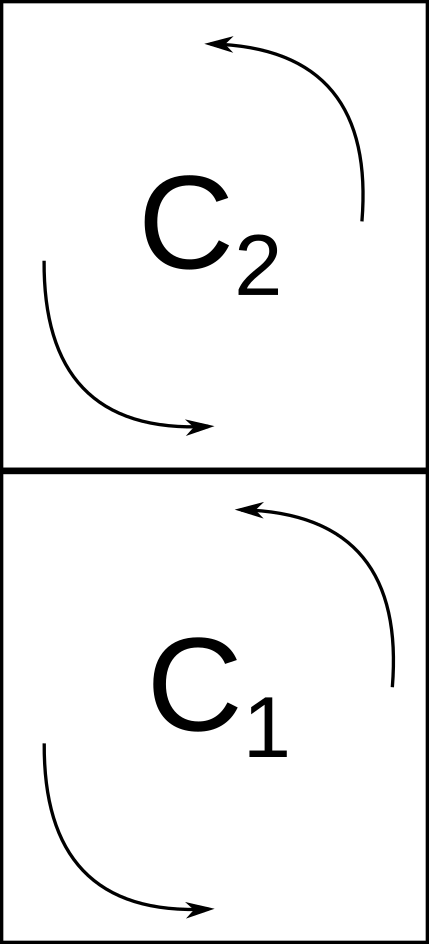
\includegraphics[width=0.7\textwidth]{../img/c1c2.png} 
\end{column}

\begin{column}{0.1\textwidth}
\Large
$\Rightarrow$
\end{column}

\begin{column}{0.2\textwidth}
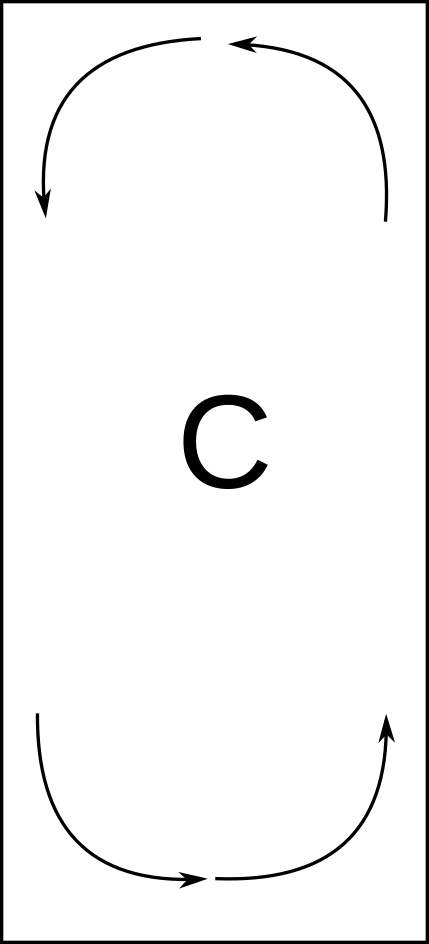
\includegraphics[width=0.7\textwidth]{../img/c.png} 
\end{column} \pause 

\begin{column}{0.4\textwidth}
\[
\oint\limits_{C_1}\vec{a}\cdot d\vec{r}+\oint\limits_{C_2}\vec{a}\cdot d\vec{r} = 
\]
\[
=\oint\limits_{C}\vec{a}\cdot d\vec{r}.
\]


\end{column}


\end{columns}
\end{exampleblock}

}



\frame{
\frametitle{Линейный интеграл от потенциального вектора}
\begin{theorems}
\parbox{\textwidth}{
Линейный интеграл вектора $ \vec{a}=\grad{\varphi} $ вдоль любой кривой $ L $, \pause  соединяющей точки $ M_0(\vec{r}_0) $ и $ M_1(\vec{r}_1) $, \pause  равен разности значений функций $ \varphi $ в этих точках.} \pause 
\end{theorems}

\begin{proof}
\parbox{\textwidth}{
Пусть кривая $L$ задана соотношением $\vec{r}=\vec{r}(s)$ и $\vec{r}_0=\vec{r}(s_0)$, $\vec{r}_1=\vec{r}(s_1)$,  \pause тогда
\[
\begin{array}{c}
\displaystyle\int\limits_{\vec{r_0}}^{\vec{r_1}}\vec{a}\cdot d\vec{r} = \pause 
\displaystyle\int\limits_{s_0}^{s_1}(a_x\dsds{x}+a_y\dsds{y}+a_z\dsds{z})ds=\\ \pause 
= \displaystyle\int\limits_{s_0}^{s_1}(\pdxds{\varphi}\dsds{x}+\pdyds{\varphi}\ds{y}+\pdzds{\varphi}\dsds{z})ds= \pause 
\int\limits_{s_0}^{s_1}\dsds{}\varphi(x(s),y(s),z(s))ds=\\ \pause 
=\varphi(\vec{r}_1)-\varphi(\vec{r}_0).
\end{array}
\]

}
\end{proof}

}


\frame{
\frametitle{Следствия из теоремы}
\parbox{\textwidth}{
\begin{exampleblock}{Два следствия теоремы:} \pause 
\begin{itemize}
\item значение интеграла от градиента функции зависит только от конечной и начальной точки и не зависит от пути интегрирования; \pause 
\item интеграл от градиента функции по замкнутому контуру равен 0  \pause (или циркуляция потенциального вектора по любому контуру равна 0).
\end{itemize}
\end{exampleblock}
}
}

\frame{
\frametitle{Критерий потенциальности векторного поля}
\scriptsize

\begin{theorems}\normalfont
\parbox{\textwidth}{
Если циркуляция вектора $ \vec{a} $ по любому замкнутому контуру равна нулю в некоторой области,  \pause  то вектор $ \vec{a} $ -- потенциальный вектор, \pause  т.е. равен градиенту некоторой скалярной функции $ \varphi $. \pause 
}
\end{theorems}

\begin{proof}
\begin{columns}
\begin{column}{0.4\textwidth}
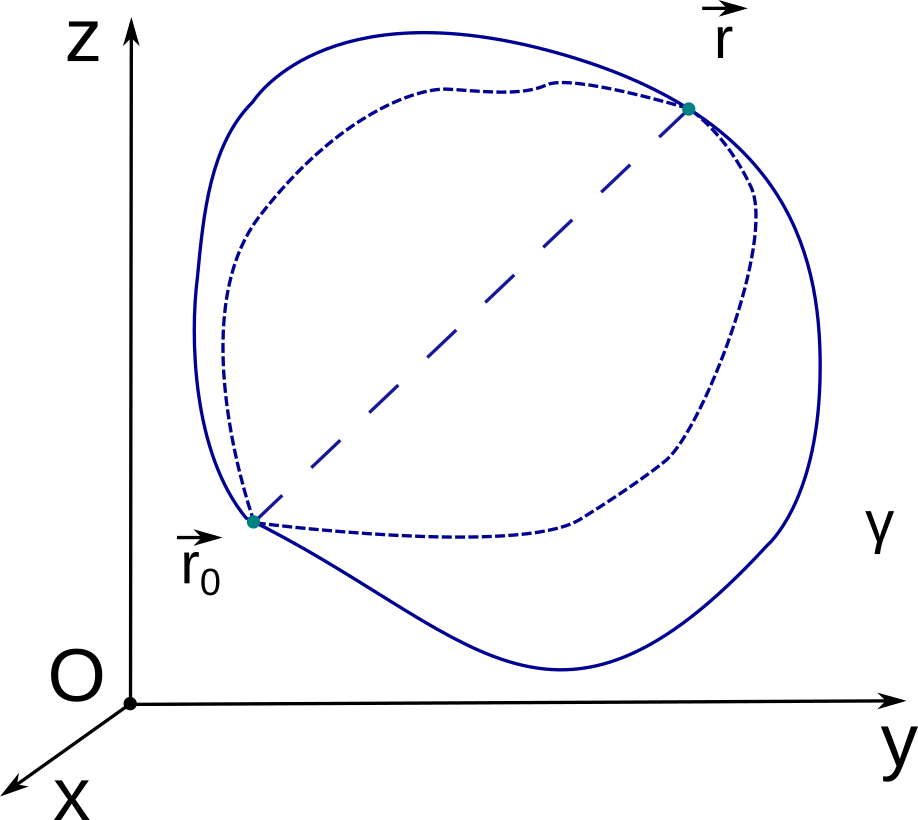
\includegraphics[width=\textwidth]{../img/circ_potential.png}
\end{column} \pause 
\begin{column}{0.6\textwidth}
\parbox{\textwidth}{

Введем $ \varphi(\vec{r}) $ вида: 
\begin{equation*}
\varphi(\vec{r})=\varphi(\vec{r}_0)+\int\limits_{\vec{r}_0}^{\vec{r}}\vec{a}\cdot d\vec{r}.
\end{equation*} \pause 
Интеграл в правой части не зависит от пути интегрирования в силу условия теоремы.  \pause 

\medskip
Полный дифференциал введенной функции
\begin{equation*}
d\varphi=\vec{a}\cdot d\vec{r},
\end{equation*}
справедлив для любых $d\vec{r}$, \pause  значит $\vec{a}=\grad{\varphi}$.
}
\end{column}
\end{columns}


\end{proof}


}



\frame{
\frametitle{Производная вдоль направления}
\scriptsize
\parbox{\textwidth}{

Пусть задана кривая $\vec{r}=\vec{r}(s)$, параметризованная параметром, связанным с длиной дуги $s$:
\[
x=x(s),\quad
y=y(s),\quad
z=z(s).
\] \pause 
Вектор $\vec{s}=\dsds{\vec{r}}$ -- единичный касательный вектор.\\ \pause 
Введем оператор
\[
\vec{s}\cdot\nabla=\cos(\vec{s},x)\pdxds{}+\cos(\vec{s},y)\pdyds{}+\cos(\vec{s},z)\pdzds{},
\] \pause 
тогда
\[ 
\pds{}a(x(s),y(s),z(s))=\vec{s}\cdot\grad{a} =  (\vec{s}\cdot\nabla) a.
\] \pause 

\begin{dfn}
\parbox{\textwidth}{
Оператор
\[
(\vec{v}\cdot\nabla)=v_x\pdx{}+v_y\pdy{}+v_z\pdz{}
\]
называется \alert{производной вдоль направления},  \pause где $\vec{v}=(v_x,v_y,v_z)$ -- заданное направление.
}
\end{dfn}

}
}

\frame{
\frametitle{Пример}

\parbox{\textwidth}{
Рассмотрим нестационарное движение жидкости, в которой определено нестационарное скалярное поле $ \varphi(t,x,y,z) $,  \pause тогда 
введем понятие местной производной
\[ 
\pdt{\varphi}= \pause \lim\limits_{\Delta t\rightarrow 0}\frac{\varphi(t+\Delta t,M)-\varphi(t,M)}{\Delta t}.
\] \pause 
Если же рассматривать изменения функции, перемещаясь вместе с жидкостью, тогда
\[ 
\dt{\varphi}= \pause \lim\limits_{\Delta t\rightarrow 0}\frac{\varphi(t+\Delta t,\vec{r}_0+\vec{v}\Delta t)-\varphi(t,\vec{r}_0)}{\Delta t}.
\] \pause 
И тогда 
\[ 
\dt{\varphi}=\pdt{\varphi}+\vec{v}\cdot\nabla\varphi,\quad 
\dt{\vec{a}}=\pdt{\vec{a}}+(\vec{v}\cdot\nabla)\vec{a}.
\]
}
}

\end{document}

